%**VARIABILI PROGETTO DA MODIFICARE****************************

\def\PROJECT		{GuFy - Guess The Film} %Nome del documento, ad esempio: Piano di Progetto
\def\SUBTITLE		{Collecting biometric measures through Gamification}

%Personale
%se ci sono più persone da indicare scrivere: {nome1, \\&nome2, \\&nome3 ecc..}
\def\AUTHOR			{\ME}

%Variabili documento
\def\TABLES		{false} %abilita - disabilita l'indice delle tabelle
\def\FIGURES	{true} %abilita - disabilita l'indice delle figure

%importa la struttura principale
\documentclass[a4paper,11pt]{article}

%Non modificare
\def\EMAIL			{filnik90@gmail.com}
\def\ME				{\mbox{Filippo De Pretto}}
\def\SERIAL			{\mbox{610673}}
\def\SUPERVISOR		{\mbox{Mauro Conti}}
\def\TUTOR			{\mbox{Fabio Aiolli}}
\def\END			{Padua, Italy, 2012.}

%*****nuovi comandi************************
%fornisce il caption per riferirsi ad una particolare sezione
\newcommand{\numref}[1]{\textsf{[\ref{#1}]}}
%formattazione per il glossario
\newcommand{\gl}[1]{\underline{#1}}
%**IMPORTAZIONE PACKAGE**************************
\usepackage[italian, english]{babel}
\usepackage[utf8]{inputenc}
\usepackage[T1]{fontenc}
\usepackage{graphicx}
\usepackage{float}
\usepackage{tabularx, array}
\usepackage{longtable}
\usepackage{chapterbib}
\usepackage[a4paper,top=3cm,bottom=3cm,left=3cm,right=3cm,bindingoffset=5mm]{geometry}
\usepackage[colorlinks=true, urlcolor=blue, citecolor=black, linkcolor=black]{hyperref}
\usepackage{booktabs}
\usepackage{totpages}
\usepackage{dcolumn}
\usepackage{epstopdf}
\usepackage{booktabs}
\usepackage{fancyhdr}
\usepackage{calc}
\usepackage{datatool}
\usepackage{listings}
\usepackage{url}
\usepackage{hyperref}
\usepackage{fancyhdr}
\usepackage{color}
\usepackage{wrapfig}

\usepackage{caption}
\usepackage{subcaption}

\definecolor{lightgray}{rgb}{.9,.9,.9}
\definecolor{darkgray}{rgb}{.4,.4,.4}
\definecolor{purple}{rgb}{0.65, 0.12, 0.82}

\lstdefinelanguage{JavaScript}{
  keywords={typeof, new, true, false, catch, function, return, null, catch, switch, var, if, in, while, do, else, case, break},
  keywordstyle=\color{blue}\bfseries,
  ndkeywords={class, export, boolean, throw, implements, import, this},
  ndkeywordstyle=\color{darkgray}\bfseries,
  identifierstyle=\color{black},
  sensitive=false,
  comment=[l]{//},
  morecomment=[s]{/*}{*/},
  commentstyle=\color{purple}\ttfamily,
  stringstyle=\color{red}\ttfamily,
  morestring=[b]',
  morestring=[b]"
}

\lstset{
   language=JavaScript,
   backgroundcolor=\color{lightgray},
   extendedchars=true,
   basicstyle=\footnotesize\ttfamily,
   showstringspaces=false,
   showspaces=false,
   numbers=left,
   numberstyle=\footnotesize,
   numbersep=9pt,
   tabsize=2,
   breaklines=true,
   showtabs=false,
   captionpos=b
}

\frenchspacing % correct spaces
\def\SCOPOPROD		{The goal of the project \gl{\PROJECT{}} is to develop an Android Application to collect informations about cellphone usage to develop new trasparent authentication method using that data.}
%**STILE PAGINA**********************************

\pagestyle{fancy}

%no indentazione paragrafo
%\setlength{\parindent}{0pt}

%intestazione
\lhead{\Large{\PROJECT{}}}
%\rhead{\includegraphics[keepaspectratio = true, width = 30px] {images/gufyIcon.png}}
\renewcommand{\headrulewidth}{0.4pt}  %Linea sotto l'intestazione
%\headsep = 35px

%piè di pagina
%\lfoot{\footnotesize{{mailto:\EMAIL}{\EMAIL}}}
\rfoot{\thepage} %per le prime pagine: mostra solo il numero romano
\cfoot{}
\renewcommand{\footrulewidth}{0.4pt}   %Linea sopra il piè di pagina

%**PRIMA PAGINA ***************************

\begin{document}		
%Prima pagina senza intestazione né piè di pagina									
\thispagestyle{empty}

%Centra il testo
\begin{center}
%\vspace{1cm}

%Titolo del PROJECT

\includegraphics[height=120px]{../documentation/img/unipd_logo.png}

\vspace{0.5cm}
{\Huge University of Padova}\\[.5pc]
{\Large Department of Mathematics}\\[.5pc]
\vspace{5 mm}
{\Huge \textbf{\PROJECT{}}}\\[.5pc]
{\Huge \SUBTITLE}\\[.4pc]
{\Large Project for BS Degree in Computer Science}\\[.5pc]
{\Large \emph{\ME{} - student number: \SERIAL{}}}\\[1pc]

%\includegraphics[height=120px]{images/gufyIcon.png}

\vspace{0.5cm}
{\Large \END}\\[3pc]

%Tabella con informazioni documento. Le seguenti variabili devono essere definite
%nel file .tex che include questa struttura
\normalsize{
	\begin{tabular}{r|l}
		\multicolumn{2}{c} {\textbf{Informations about the document}} \\
		\midrule
		\textbf{Author} 				& \AUTHOR \\
		\textbf{Supervisor} 			& \SUPERVISOR \\
		\textbf{Internal tutor} 		& \TUTOR \\
	\end{tabular}
}

%Fine zona centrata
\end{center}

%Indica che è finita la pagina corrente ed inizia la prossima
\newpage
%si usa la numerazione romana per gli indici e la tabella delle modifiche
\pagenumbering{Roman}
%************************************************


\newpage
\thispagestyle{empty}
\mbox{}
\newpage

\newpage
%************************************************
%importa i vari indici
%************************************************
%Inserisce il link all'indice
\addcontentsline{toc}{section}{Index}
\tableofcontents
\newpage

%se è stata impostata a true la variabile per la lista delle tabelle, la mostra
\ifthenelse{\equal{\TABLES}{true}} 
{\listoftables \newpage}{}

%se è stata impostata a true la variabile per la lista delle figure, la mostra
\ifthenelse{\equal{\FIGURES}{true}}
{\listoffigures \newpage}{}

%da qui comincia la numerazione normale
\pagenumbering{arabic}

%imposta il formato di visualizzazione
\rfoot{\thepage ~of~\pageref{TotPages}}

%**********   Inizio delle "section"   ********************************

\newpage
\thispagestyle{empty}
\mbox{}
\newpage

\hspace{1cm}
\begin{center}
\section*{Abstract}
\end{center}
Recently, researchers of the ``Mind How You Answer Me!'' project (from now on: MHYAM \cite{MHYAM}), proposed a biometric method to transparently authenticate an user when answering a phone call. 

Even though the outcomes are promising, the data-set used is of only 10 users. To confirm the results of this research is needed a bigger data-set. For this goal, we have created a new Android application: GuFy (Guess the Film). 

This is a videogame, where the user has to guess what is the right movie, after listening to a short track of it. Using the Android market we can reach a big number of people and is important to induce them to continue to play. We hope to track some of the players also for a long time. In this way we can also see how the human biometric changes during the time.

\newpage
\thispagestyle{empty}
\mbox{}
\newpage

\section{Introduction} 	
The MHYAM Project \cite{MHYAM} has given an important contribution to the development of solutions to transparently authenticate the users using their phone call behavior. However, the solution has been tested using a small data-set of 10 people. Furthermore, the testing application used resulted in a small interest for the user, because it simply asks to act like she would during a phone call. To reduce the errors of the algorithms is important to retrieve a wider data-set and to do that we used a recently proposed technique that is gaining a lot of consensus among the companies and researches: Gamification \cite{website:gamification-wikipedia}. 

\begin{figure}[H]
\centering % per centrare l'immagine (opzionale)
\includegraphics[width=\textwidth]{images/gartner-hypecycle.png}
\caption{Gartner's hype cycle - 2011}
\label{fig:GamificationHypeCycle}
\end{figure}

This idea works by \textit{making technology more engaging, by encouraging users to engage in desired behaviors, by showing a path to mastery and autonomy, and by taking advantage of humans' psychological predisposition to engage in gaming} \cite{website:gamification-wikipedia}.

As you can see in Figure \ref{fig:GamificationHypeCycle} in Gartner's hype cycle, Gamification has become popular in these days. There aren't already a lot of working examples, but the few ones are really promising as you will see in Section \ref{sec:related}.

Gamification is still in its early steps but it is one of the technologies more promising since there aren't already a lot of competitors and it will become mainstream in the near future.

Using this system, we want to reach our goal that are to:
\begin{itemize}
\item spread the application and get a lot of users (and their data);
\item collect a wide range of data for each user that uses the application, and not just one record or two, as in the application already developed;
\item check the quality of the data for transparent authentication.
\end{itemize}

To do that, has been developed an Android videogame where:
\begin{enumerate}
\item the user has to click a button to start an audio track;
\item a track starts with a part of a movie. To listen it, she has to put the phone next to the ear. The volume is set so that it is the only way to hear the track;
\item when the track ends, she has to put the phone down and guess which movie she heard.
\end{enumerate}

To avoid bad track recording, has been also disabled the head-set, so the user can't simply listen the track while she is looking at the phone and the buttons to answer are enabled only after 3 seconds after that the track has started. At the first start of the game, has also been suggested the right way to use the application, i. e. to place the phone next to the ear to listen the track, before answering.

In this way, the user isn't induced to simply look at the phone listening to the track, but she ears the track and then answers, recording a track similar to what is recorded during a phone call.

%%%%%%%%%%%%%%%%%%%%%%%%%%%%%%%%%%%%%%%%%%%%%%%%%%%%%%%%%%%%%%%%%%%%%%%%%%%%%%%%%%%%%
\subsection{Problem Description}
\label{sec:problems}
For the MHYAM project \cite{MHYAM} is important to have a valid and wide data-set, to test the algorithms and create applications that use them. Until now, it has been developed only one simple Android application that collect the data, asking the user to act as she would during a phone call. With this application, the project has reached important conclusions, i.e. the human behavior when answering a call is a biometric measure, because the user tends to act always in the same way when answering. Furthermore, two different users usually have two different patterns.

However, the program developed has still around 2\% of False Alarm Rate (FAR) and around 1.5\% Impostor Pass Rate (IPR), that are great results but need to be further verified with a bigger dataset and may be improved with further experiments and other similarity algorithms.

Another problem not solved in the MHYAM project is that the users tested knew exactly what they were doing: a phone call test. In this way, they may be induced to act always in the same way, also for ``consistency''. It is indeed typical that a human being tends to act always in a same way, both as actions and behavior, to be consistent. The society tells us that someone that vary a lot her behavior is not someone ``normal'', so when you are under a test and someone is watching you, your brain automatically tries to be as more consistent as possible \cite{influence}. 

Finally, the user may enter in a sort of ``self-fulfilling prophecy''. If the person knows (or imagines) the goal of the project, i.e. the  confirmation that a human being has always the same behavior, she may be inducted to act as if it is really true \cite{influence}.

\subsection{Contribution}
\label{sec:contribution}
The development of the GuFy application has indeed the goal to solve or reduce some of the problems shown in the Section \ref{sec:problems}.

The use of a game in the tests leads to more natural acts, similar to what the user normally does during a phone call. As we speak, the application has been successfully developed and is going to be uploaded on the Android Market. However, we think that the results would be the same as in the MHYAM project \cite{MHYAM}, because an user still have a sort of ``internal consistency'', so although there is nobody watching the user, she still should act in the same way but probably less than in previous tests. So we imagine that the outcomes of this data-set would be less good as in the MHYAM project. 

However, the other questions that remain to be answered are: will the user act in the same way during all her life? And in every situation? Will she change her behavior if her mood changes? (for example: when she wins or looses). With this application we may also track the history of the user to see how her behavior changes, how fast and in which typical ways. 

So, with this project, we can retrieve a lot of informations:
\begin{itemize}
\item user's behaviour during a phone call;
\item how user's behaviour changes during her life;
\item Facebook data and connections.
\end{itemize}

Indeed, to play the game, is required to login with Facebook. In this way is possible to collect useful informations about the users playing and how that characteristics influences the various people. For example, has women different tracks from men? Does the country or the city influence the way that the poeple answer the phone?

It will be possible to answer to these questions because from the first version of the application these data are automatically stored, without bother the user. Furthermore it is possible to analize these data also for other social researches and to use the user's token, automatically stored by the application, for getting other data and useful informations about the user, without creating a new application.

The second goal is particularly ambitious, and can be achieved only in a long period, but I am interested in the maintenance of the application and in the developing of a free and open solution to develop more games quest-based. The application was indeed designed thinking to a common quest and not only for quests about movies.

This project is in this way important because it can lead to an easy development of a series of application that uses Gamification to retrieve useful data and to teach something useful in the process. For example, it can be used to retrieve data about the user's face for testing new face or ear recognition algorithms or to teach programming languages, creating a database of codes with whom the user has to deal with in the typical ``does it compile?'' test, that is common in the main three courses of programming at the University of Padua.

This can lead in a wide network of devices connected and that give us important informations from the sensors but also from their Facebook accounts, that can be effectively used for research.

\subsection{Organization}
This document presents the project as it has been developed during the time. So, first of all, there is an overview of the related works, in Section \ref{sec:related}. This project was indeed a derivation of the research development in the fields of biometric authentication and gamification. After that, there is Section \ref{sec:businessAnalysis} that is dedicated to the business analysis of the members of project, of our competitors and of our future ``clients''. The application will be released for free, but it has to be of some interest to be downloaded.

In Section \ref{sec:requirements} we will show the requirements outlined after we have chosen the project and we have analysed the actual situation. These requirements will be then developed into a planning solution, as you will see in Section \ref{sec:planning}. In this section there are all the diagrams of the classes of the project.

We will then continue with the description of the technologies chosen. in Section \ref{sec:technologies} This was a main decision of the project, since it has influenced all the development and the timing. After that, we will see how everything we planned has been actually created. This has been done in Section \ref{sec:actualApplication}.

After the creation of the project, in Section \ref{sec:validation} we describe how we checked the quality of what we have produced.

Finally, there is the project time-line, Section \ref{sec:timeline} and the final assessment, Section \ref{sec:finalAssessment} describing how the project has been planned and how it developed over the time.

We have also added two appendixes after the conclusions, that are how you can install the software, Section \ref{sec:installSoftware} and License \& Legal aspects, Section \ref{sec:legal}.

\newpage

%%%%%%%%%%%%%%%%%%%%%%%%%%%%%%%%%%%%%%%%%%%%%%%%%%%%%%%%%%%%%%%%%%%%%%%%%%%%%%%%%%%%%
\section{Related Work}
\label{sec:related}

Authentication for mobile devices is an old issue and there have been a lot of proposals to solve the problem. The most common solution is the use of PIN based method that are still widely used nowadays. The main problem of this solution is that it is not transparent and the user must remember the numbers: fact that leads to the use of simple numbers to remember but also to break or to the deactivation of the feature \cite{1284685}. Another typical method is the use of graphical figures as passwords but the problems remain the same \cite{USENIX_Security_99}.

To solve these problems, research has moved to biometric measures that are hard to break since their ``secret'' is inside the human behavior and it is hard to spy and reproduce. 

Biometric measures are classified into two main categories: physiological biometrics and behavioral biometrics \cite{621409}.

Physiological biometrics identify the user based on her physiological features. They include: face recognition [4], fingerprint recognition \cite{621409}, external ear shape recognition \cite{1296543}, internal acoustic ear shape recognition \cite{1104752} (i.e. measuring the shape of the ear channel using acoustic data). 

These methods however have the following issues:
\begin{itemize}
\item non transparent usage;
\item performance are heavily influenced by external factors such as illumination, position or occlusion \cite{621409}; 
\item lack of required hardware on current smartphones.
\end{itemize}

About these methods, must be cited that external ear shape recognition \cite{1296543, face-ear-images} has a good recognition rate (around 90\%) and internal acoustic ear recognition \cite{1104752} has an Equal Error Rate of around 5.5\%. However, these methods are influenced by factors like hair, hats or veils. At the same time, the camera should be at a distance appropriate to get the correct focus on the target, so it might be impossible to get a valid photo when, for example, the user answers a call. In the previous tests, indeed, there was a specific setup for capturing the image and an active participation of the user (e.g. uncovering the ears from the hair). So this method is not transparent at all and needs time to get a good result.

Within physiological biometric measures, methods that do not suffer much of obstruction problems are fingerprint recognition \cite{621409} and internal ear recognition. However, the first one needs a scanner and it is not transparent, the second one a device that is placed in the ear to emit acoustic signals and a microphone needs to be attached to the smartphone.

The other classification of biometric measures is the one of behavioral biometrics, where user is identified based on her behavioral features: e.g. keystroke dynamics \cite{Gunetti:TISSEC:2005}, voice pattern \cite{348995} or gesture (e.g. the user's walking pattern \cite{gait}). 

All these methods suffer the fact that they need time to understand if the user's behavior is really different or not. For example, in order to recognize the user from her walking pattern \cite{gait}, the user would have to walk first, before
the device is able to figure out whether she is the correct user or not. For keystroke dynamics the user has to type a phrase, e.g. up to over 100 characters before recognition can be performed \cite{Joyce:CommACM:1990, Leggett:IJMMS:1988, Gunetti:TISSEC:2005}.

Similarly, for voice recognition the user would have to output some predefined phrases, or sounds, before being authenticated \cite{348995}.

Recently, has been released new mechanisms that aim to identify the user basing on a secret movement pattern \cite{accelerometer} (e.g. moving the phone to draw an ``8'' in the air, where ``8'' is the secret). The security obtained is high. However, there are the same problems found for PINs or graphical images (simple secrets and easy to spy and replicate).

The MHYAM project \cite{MHYAM} presented a method that solves the problems of the cited methods. The proposed solution, as already said, consists in measuring the movement pattern performed by a user while answering (or placing) a phone call. 

The observations were that, differently from the solution in \cite{accelerometer}, in the MHYAM project the secret is not the movement itself (e.g. the ``8'' drawn in the air) but it is the biometric measures of a specific user's movement. So, even if an adversary spies how the user answers the phone, she is not able to replicate the movement in a way such that it can replicate the biometric features of the correct user.

The project proposed to measure movement patterns using both the accelerometer sensor and the orientation sensor. Also, has been proposed a specific way of combining different authentication methods (based on different sensors and different recognition algorithms) reaching low FAR (False Alarm Rate) and IPR (Impostor Pass Rate) \cite{multimodalBiometrics}.

Results show therefore that the method is effective and the performance is comparable to that of other transparent authentication methods, like face or voice recognition. However, the data-set used is limited and the goal of the GuFy project is to retrieve a more wide data-set to test the proposed technique. 

To do that we have implemented a new application, based on the idea of Gamification. This application will collect the data trough a simple game, amusing the user while she's giving us important informations. In this way, we believe that the dataset collected with GuFy will reflect the real actions that an user does placing a phone call and this will overcame the limitations listed in Section \ref{sec:problems}. 

Other examples of gamification in research can be found in \cite{vonAhn:2004:LIC:985692.985733} that describes as it has been developed a game to do a tedious work such as labeling images. In this way, what was tedious becomes something fun and this is proven by the numbers of users that have played and the fact that this game has been bought by Google.

The results were indeed extraordinary, people enjoyed to play that game doing something useful for the research, getting anything else than the fun in exchange. The most important fact was also that, due to the construction of the game itself, the outcomes gained with the game were effective and the results of a query with this system were a lot more useful than in previous systems that used the text around the images or the name of the files to tag them.

Our focus has been to make the same thing in our project, developing challenges for the users, high scores and rewards to make the game as more fun as possible to get a precise profile of the user.

An issue that in \cite{vonAhn:2004:LIC:985692.985733} has been solved in a great way, is the problem that someone can cheat and record some invalid words for some photos that have nothing to do with them. We may have the same problem, because mobile devices are typically borrowed to friends and relatives that may ``try'' the application without creating a new user only for a ``quick run''. However, the ``quick run'' will record invalid patterns that have nothing to do with the user itself. This situation may happen just few times, but this will make the data-set not valid. 

To avoid these situations we have chosen the facebook login that checks user's identity before proceeding. In the future releases of the project, when the data retrieved will be enough to judge if the method is effective, we will also use the DTW algorithm to detect when the user changes, prompting another login screen.

\newpage

\section{Business Analysis}
\label{sec:businessAnalysis}

In this section will be described the current situation of the Android Market. In this way we can see who are our competitors, analyse their solutions and understand why the have or don't have success and what is the focus that we should have to get a better outcome than any other competitor already on the market.

We should also focus on what is our value proposition, understanding the real needs of our costumers and match what they really want. 

We has also the ``problem'' that we are a multi-sided platform, so we have to match both the needs of researchers that needs the users' data and users that want an amazing application to play with. 

For this analysis, we will follow what has been taught in the ``Gestione delle imprese'' class, following international standards \cite{article:ElementsOfUserExperience}, \cite{market-driven-management}.

\subsection{Get ready}
To start with the project we have to identify who are our costumers. This will be better done later when we will find out the personae that will represent our costumer segment.

However, the development team will be:
\begin{itemize}
\item \textbf{Me}. I have no particular movie skill, but I know what can and what cannot be done;
\item \textbf{Researches}, in particular: Dr. Mauro Conti, Dr. Fabio Aiolli and the CRêPE team. They have no particular movie skill, but they need the data of the project and have a great experience on developing new research projects;
\item \textbf{Movie experts}, in particular: Giulia Nespoli and Alessandro Pinarello. The first one, is a student at the DAMS of the University of Venice and has a long-time experience and strong passion on movies, old ones too. The second one is a student at computer science here at the University of Padua. He has grown in his father's video store and has developed a strong passion about movies;
\item \textbf{Common people}, in particular: Teresa Colangelo and Nicolò De Pretto (my brother). Our target are not only movie experts, but also common people. They will help with alpha and beta testing, usability tests and comments about the project.
\end{itemize}

This group allows us to have a variety of opinions, in order not to focus only on one needs forgetting the ``costumers'' or the researches that need usable data.

\subsection{Theme}

We will focus on these technologies to make the product more engaging:
\begin{itemize}
\item \textbf{Data Analytics:} after the product's release, we expect that we will get a big amount of data to process and analyse. In this way we can find useful information for researchers;
\item \textbf{Gamification:} we will create a videogame to make the product engaging and fun for our costumers;
\item \textbf{Mobile:} we will develop a mobile application to do that;
\item \textbf{Social:} we will try to make the application as more social as we can to spread it on the web.
\end{itemize}

This will be done in two ways:
\begin{itemize}
\item \textbf{B2C} (\textit{Business to Consumer}): this means that we will initially create the movie-database with the help of the team outlined before;
\item \textbf{C2C} (\textit{Consumer to Consumer}): this means that our focus is to create a structure that, after the initial input, can grow and develop without the help and the lead of administrators.
\end{itemize}

The B2C solution is already completely working, the C2C solution is though only a project and our focus for the future. The reason is that we need to create a more engaging platform also server-side to gain new ``quest authors'', using Gamification. This couldn't obviously be done in the 300 hours for the project, but it will be done in the next months. 

\subsection{Competitors}

\begin{center}
``It's all about predicting competitors, either competitor behavior or competitive environment behavior.'' (Wayne
Rosenkrans)
\end{center}

First of all, we have to find out who are our competitors and understand what are their pros and cons to create a product that differentiates from the others. This has been done according to the most common standards about competitors analysis. \cite{market-driven-management}

\subsubsection{Movie Master}

\begin{figure}[H]
\centering % per centrare l'immagine (opzionale)
\includegraphics[height=150px]{../documentation/img/business_analysis/movieMaster.jpg}
\caption{Movie Master screenshot}
\label{fig:movieMaster}
\end{figure}

\begin{description}
\item[Application Name:] Movie Master;
\item[Developer:] Boyan\_Soft;
\item[Developer importance:] high;
\item[Project description:] this project has been born after the success of Boyan\_Soft millionaire application. As you can see in Figure \ref{fig:movieMaster}, the format is more or less the same, what changes is only the topic that are the movies. So, you have a screenshot of the film selected and you can use some helps (such as in millionaire) and guess. The graphic is simple but clean and usable;
\item[Customer Segments:] B2C. This product doesn't allow you to upload new images to play with. However, the database seems large enough to be fun and not repetitive. The target however is only one: common people. The films given are pretty new and it is hard to find something older than 1995-2000, while real experts love every kind of movies, not only new ones. So: \textbf{mass market};
\item[Pros:] Strong brand (it has already a lot of downloads), clean graphic, engaging game, usable, enough wide database. Openfeint connection available;
\item[Cons:] No C2C, only new films, difficulty not selectable, when you loose you have to start from the beginning;
\item[Guessing system:] it is based on a screenshot of the movie. You have some hints that you can use. When you make a mistake you have to start from the beginning;
\item[Requires internet connection:] No;
\item[Downloads:] 50.000 - 100.000;
\item[Ranking:] 4.3/5;
\item[Language:] English;
\item[Dimensions:] 10Mb;
\item[Adds:] No;
\item[Price:] Free.
\end{description}

\subsubsection{What movie is that?}

\begin{figure}[H]
\centering % per centrare l'immagine (opzionale)
\includegraphics[height=150px]{../documentation/img/business_analysis/WhatMovieIsThat?.jpg}
\caption{Quiz Film screenshot}
\label{fig:whatMovieIsThat}
\end{figure}

\begin{description}
\item[Application Name:] What movie is that?;
\item[Developer:] Android Projects DJ;
\item[Developer importance:] low;
\item[Project description:] this project is similar to ther other ones but more difficult to play. You have not to guess the title of the film, you have to write it. The format however is the same: screenshot and guess;
\item[Customer Segments:] B2C. \textbf{mass market};
\item[Pros:] good graphic, localization in English and Spanish;
\item[Cons:] Guess the title might be more engaging for someone, but it is way more difficult. The English localization is not so well done but usable;
\item[Guessing system:] Screenshot and guess writing the title. You have no hints. You have all the film to guess like an Advent-Calendar and you can jump to the one you want, so you have not to start from the beginning each time;
\item[Requires internet connection:] No;
\item[Downloads:] 5.000 - 10.000 (free version) / 10 - 50 (payed version);
\item[Ranking:] 3.1/5;
\item[Language:] English / Spanish;
\item[Dimensions:] 636kb;
\item[Adds:] No;
\item[Price:] Free version and payed version (0,76 Euro).
\end{description}

\subsubsection{Movie Hangman}

\begin{figure}[H]
\centering % per centrare l'immagine (opzionale)
\includegraphics[height=150px]{../documentation/img/business_analysis/movieHangman.jpg}
\caption{Movie Hangman screenshot}
\label{fig:movieHangman}
\end{figure}

\begin{description}
\item[Application Name:] Movie Hangman;
\item[Developer:] Hamish Tushar;
\item[Developer importance:] low;
\item[Project description:] this project has something new respect than the previous ones. In particular, you have to guess the film's name in ``hangman'' style, i.e. you have to select the letters you want to compose the name and every time you fail, the program draws a new part of the body of the hangman.
\item[Customer Segments:] B2C. \textbf{mass market};
\item[Pros:] simple and usable graphic. The game is engaging. You have not to start from the beginning if you lost;
\item[Cons:] Guess the title might be more engaging for someone, but it is way more difficult. However the hangman system is much better than writing the whole title without help;
\item[Guessing system:] Hangman system and hints when you are loosing;
\item[Requires internet connection:] No;
\item[Downloads:] 1.000 - 5.000;
\item[Ranking:] 4.9/5;
\item[Language:] English;
\item[Dimensions:] 721kb;
\item[Adds:] Yes;
\item[Price:] Free.
\end{description}

\subsubsection{Guess Movies}

\begin{figure}[H]
\centering % per centrare l'immagine (opzionale)
\includegraphics[height=150px]{../documentation/img/business_analysis/guessMovies.jpg}
\caption{Guess Movies screenshot}
\label{fig:guessMovies}
\end{figure}

\begin{description}
\item[Application Name:] Guess Movies;
\item[Developer:] Demansol;
\item[Developer importance:] high;
\item[Project description:] this project is similar to the first one. Screenshot and guess, but the screenshot is hidden below some stones that you can remove using the help-button. Thing that gives you less points. This game has also more feature than the others and is more engaging;
\item[Customer Segments:] B2C. \textbf{mass market};
\item[Pros:] the graphic is not particular but easy to use. You can select the difficulty. There are ranking for the two difficulties available. The help system is quite interesting and well done. After that you guess or loose, the game gives you information about the film itself. You haven't to start from the beginning if you make a mistake;
\item[Cons:] The graphic could be better. The ranking can be only one, giving less points to who plays the easy-mode. Only two levels of difficulty;
\item[Guessing system:] Screenshot and guess system but with stone-system;
\item[Requires internet connection:] No;
\item[Downloads:] 10.000 - 50.000;
\item[Ranking:] 3.2/5;
\item[Language:] English;
\item[Dimensions:] 12Mb;
\item[Adds:] No;
\item[Price:] Free.
\end{description}

\subsubsection{Movie Guess - Freesoul}

\begin{figure}[H]
\centering % per centrare l'immagine (opzionale)
\includegraphics[height=150px]{../documentation/img/business_analysis/movieGuess.jpg}
\caption{Movie Guess screenshot}
\label{fig:movieGuess}
\end{figure}

\begin{description}
\item[Application Name:] Movie Guess;
\item[Developer:] Freesoul;
\item[Developer importance:] low;
\item[Project description:] same format as the previous ones. Screenshot of the film and you have to guess the film selected. However, the game is designed better than the others;
\item[Customer Segments:] B2C. \textbf{mass market};
\item[Pros:] really good graphic. Simple but elegant. The game is simply to use and to understand. Few features but well done. You have not to start from the beginning if you make a mistake; you have only one 50\% and 50\% like millionaire as hint. Openfeint connection enabled;
\item[Cons:] Few features available and simple. Becomes boring soon;
\item[Guessing system:] Screenshot and guess system;
\item[Requires internet connection:] No;
\item[Downloads:] 1.000 - 5.000;
\item[Ranking:] 4.1/5;
\item[Language:] English;
\item[Dimensions:] 4,3M;
\item[Adds:] No;
\item[Price:] Free.
\end{description}

\subsubsection{Guess Who}

\begin{figure}[H]
\centering % per centrare l'immagine (opzionale)
\includegraphics[height=150px]{../documentation/img/business_analysis/guessWho.jpg}
\caption{Guess Who screenshot}
\label{fig:guessWho}
\end{figure}

\begin{description}
\item[Application Name:] Guess Who;
\item[Developer:] Sergey Babochkin;
\item[Developer importance:] low;
\item[Project description:] this is a little different. Here we have to guess the actor and not the film. This is interesting also because there is a practise mode where you can make as many mistakes you want and a challenge mode where when you fail you have to start from the beginning;
\item[Customer Segments:] B2C. \textbf{mass market};
\item[Pros:] the best graphic seen until now. Practise mode is an interesting feature. Well designed. A bit boring however;
\item[Cons:] Only actors and not movies. Few features and no hints;
\item[Guessing system:] Screenshot and guess system;
\item[Requires internet connection:] No;
\item[Downloads:] 10.000 - 50.000;
\item[Ranking:] 3.0/5;
\item[Language:] English;
\item[Dimensions:] 4,1M;
\item[Adds:] No;
\item[Price:] Free.
\end{description}

\subsubsection{Competitors positioning}
\begin{figure}[H]
\centering % per centrare l'immagine (opzionale)
\includegraphics[width=\textwidth]{../documentation/img/business_analysis/CompetitorPositioningTechniquesEngaging.png}
\caption{Competitors positioning based on Techniques/Hints and engaging}
\label{fig:competitorsPositioningTechAndEngaging}
\end{figure}

In Figure \ref{fig:competitorsPositioningTechAndEngaging} we can see the positions of competitors based on the number of techniques to make the user guess the film and how much fun is the game itself.

With this graphic we see that if you have less techniques or hints, your game is less engaging than the others, but that it is not the only thing that is important.

\newpage

\subsection{Personae}
\label{sec:personae}

\begin{center}
\textit{``A persona is a fictional character constructed to represent the needs
of a whole range of real users. By putting a face and a name on the
disconnected bits of data from your user research and segmentation
work, personas can help ensure that you keep the users in mind
during the design process.''} \cite{article:ElementsOfUserExperience}
\end{center}

As explained in Elements of User Experience, we have analysed the different kind of people involved in the project. In this way we are sure to match all the needs that the different people want, without focusing too much on one or another profile.

\subsubsection{Researcher}

\begin{figure}[H]
\centering
\includegraphics[keepaspectratio = true, width = 120px] {images/researcher.jpg}
\caption{Martin - Researcher}
\label{fig:researcher}
\end{figure}

\begin{description}
\item[Name:] Martin;
\item[Età:] 42;
\item[Gender:] Male;
\item[Profession:] Security expert;
\item[Degree:] PhD in mathematics;
\item[Focus:] find useful data for research purpose, in particular about transparent authentication. Martin wants also that the application would be successful to collect more data and to show how serious games can be used for research purposes. He may also be interested in Facebook data for other security analysis;
\item[Fears:] Martin is afraid of loosing time in a project that migh turn useless or that doesn't retrieve useful information;
\item[Channels:] he meets new people mainly in conferences and at the university. He interacts with students and other researchers. Tony can be reached with traditional channels (TV, newspapers, etc.) but also through technical sites;
\item[Influence:] his opinion is important and he might influence a lot of people at lesson, in conferences and at the university speaking with other researchers.
\end{description}

\newpage

\subsubsection{Movie expert}

\begin{figure}[H]
\centering
\includegraphics[keepaspectratio = true, width = 120px] {../documentation/img/business_analysis/movieExpert.jpg}
\caption{Isabelle - Movie expert}
\label{fig:movieExpert}
\end{figure}

\begin{description}
\item[Name:] Isabelle;
\item[Età:] 22;
\item[Gender:] Female;
\item[Profession:] Artist student;
\item[Degree:] High school;
\item[Focus:] she wants to find out a new game that matches her interests. She wants to create new tracks to misure her ability with other movie experts and maybe create a selection of tracks with her name to challenge other movie experts. She is interested on the creation of high-level connections with other experts. She wants also to learn something new, in particular she wants informations about the films that she doesn't guess. She will be satisfied if the movies uploaded will be good rated and if she has a high rank;
\item[Fears:] she is afraid of the fact that research needs will lead to the creation of a less satisfacting game. She is also afraid to loose time in a game without a huge database to play with and that she can't find experts in this game;
\item[Channels:] she likes watching TV. She spends some time on social media, such as facebook or twitter, where she can find useful informations. She may follow also websites such as ``comingsoon'' and sites/forums for movie experts;
\item[Influence:] she has a big influence on people like her. Also common people may be listening to her, but only if they share some movie category, otherwise they may not trust her judgment about what is fun and what not.
\end{description}

\newpage

\subsubsection{Common person}

\begin{figure}[H]
\centering
\includegraphics[keepaspectratio = true, width = 120px] {images/commonPerson.png}
\caption{Eric - Common person}
\label{fig:commonPerson}
\end{figure}

\begin{description}
\item[Name:] Eric;
\item[Età:] 28;
\item[Gender:] Male;
\item[Profession:] Student;
\item[Degree:] University student;
\item[Focus:] Eric is interested in movies and he watches them in his free time. However, he has not so much time to waste, so he wants something easy to play with and that makes you earn a lot of points fast. Furthermore, he wants something engaging and not boring or too repetitive. So the game should be progressive and with things that will be unlocked while he continues to play;
\item[Fears:] Eric is afraid of loosing time in something boring or that is not engaging because it is too repetitive. He may fear the fact that other people find out that he looses a lot of time with mobile games;
\item[Channels:] he has not so much time for TV but he watches the news. His main channels are social media, news websites and newspapers. He is also highly influenced by his friends and family;
\item[Influence:] Eric has a reduced influence about this topic over other people. Indeed, he is not an expert, but his friends may try the application when he shows them the game. However, he may not want to spread the game, because he wants to keep his image of a serious guy. For this reason, pointing out that the game is important for research might be important and useful.
\end{description}

\newpage

\subsection{Conclusions}
The market has already some solutions similar to what we are proposing, so it will be harder to gain new users. 

However, our solution has different features than the solutions proposed. In first place the C2C solution is something new and never proposed, so the user might be more interested playing our game to create new contents for the game, when this feature will be released.

Furthermore, every solution includes only screenshot and not short tracks of the movie. Thing that may make the game more engaging. Important is also the graphic that must be easy to use, since when you are playing you have no time to waste.

In conclusion, there are similar solutions but the market may answer in a positive way the entrance of a new application of higher quality.

\newpage

\section{Requirements Analysis}

In this section we will show the user requirements. I outlined these requirements having meetings with Dr. Mauro Conti and the other people that helped with their feedbacks about the project.

Since the project's development will continue after this thesis, we have outlined the necessarily requirements first and then described the desirable ones and, finally, the optional ones. The last two types of requirements aren't strictly needed and, as for example with the multiplayer requirements, haven't been described in the use cases, since was highly improbable to accomplish it in time.

We have so decided to described the most needed requirements, knowing that some of them would be accomplished only in case of extra time spent on the project.

In the feasibility study, we found out also some legal requirements. We process delicate data, that it is necessary to protect with a secure client-server solution. More about it will be described in the Planning part, but we have to consider it also as a ``legal'' requirement.

\subsection{Use cases}
What follows is a concise description of the main use cases developed for the project. 

\subsection{Mobile Application}
\begin{figure}[H]
\centering % per centrare l'immagine (opzionale)
\includegraphics[width=300px]{images/usecase/GufyMobile.png}
\caption{Mobile application use case}
\label{fig:GufyMobile}
\end{figure}

\begin{description}
	\item[Actors:] The \textit{user} of the mobile application, the \textit{user logged} in the application and the two servers (or, in our case, the two collections) i.e. the \textit{Game Server} and the \textit{Biometrics server};
	\item[Description:] In Figure \ref{fig:GufyMobile} is displayed the main screen of the system. The user has the ability to log-in, see a wizard or to share his interest on our application. The user logged has further possibilities that allows him to use the settings, see the ranking, play single or multiplayer and to download the tracks;
	\item[Scenario illustration:]
	
		\begin{description}
			\item[UC\_1.1:] [necessary] The user must have the ability to log in the system;
			\item[UC\_1.2:] [optional] The program should allow to view a simple wizard about itself;
			\item[UC\_1.3:] [optional] The user should have the possibility to share the application in the most common social networks;
			\item[UC\_1.4:] [desirable] The program should have a section dedicated to the settings;
			\item[UC\_1.5:] [desirable] The user should have the possibility to see his ranking and the ranking of other users;
			\item[UC\_1.6:] [necessary] The Single Player is the use case dedicated to the game;
			\item[UC\_1.7:] [optional] The Multiplayer is the use case where one player plays with other players instead of against the program;
			\item[UC\_1.8:] [optional] The last requirements shows the need to download the tracks to play offline.
		\end{description}

\end{description}

\subsubsection{Social}
\label{sec:social}
\begin{figure}[H]
\centering % per centrare l'immagine (opzionale)
\includegraphics[width=300px]{images/usecase/Social.png}
\caption{Social use case}
\label{fig:SocialMobileUseCase}
\end{figure}

\begin{description}
	\item[Actors:] The \textit{user} and all the systems to share the application installed in the device;
	\item[Description:] In Figure \ref{fig:SocialMobileUseCase} is shown the use case about the social interaction of the application. This option allows the user to share and rate the application.
\end{description}

\subsubsection{Settings}
\label{sec:settings}
\begin{figure}[H]
\centering % per centrare l'immagine (opzionale)
\includegraphics[width=300px]{images/usecase/Settings.png}
\caption{Settings use case}
\label{fig:SettingsUseCase}
\end{figure}

\begin{description}
	\item[Actors:] The \textit{user} of the mobile application, the \textit{user logged} in the application and the \textit{Game Server};
	\item[Description:] In Figure \ref{fig:SettingsUseCase} is shown the use case about the settings. They have been implemented as a fragment, as you can see in Figure \ref{fig:settings}. However, now there are no statistics to show and the language is deducted automatically by the system, so at this step they are of no particular interest;
	\item[Scenario Illustration:]
	
		\begin{description}
			\item[UC\_1.4.1:] [necessary] The user needs to be able to change language. The languages needed should be at least italian and english;
			\item[UC\_1.4.2:] [desirable] The user should be able to select his favourite categories;
			\item[UC\_1.4.3:] [desirable] The user should be able to change account if she wants;
			\item[UC\_1.4.4:] [optional] The user should be able to view his statistics.
		\end{description}
\end{description}

\subsubsection{Single Player}
\label{sec:singlePlayer}
\begin{figure}[H]
\centering % per centrare l'immagine (opzionale)
\includegraphics[width=300px]{images/usecase/SinglePlayer.png}
\caption{Single Player use case}
\label{fig:SinglePlayerUseCase}
\end{figure}

\begin{description}
	\item[Actors:] The \textit{user} of the mobile application, the \textit{user logged} in the application and the \textit{Game Server};
	\item[Description:] In Figure \ref{fig:SinglePlayerUseCase} is shown the use case about the Single Player. This is the most important window and describes the actual game. The user can listen to the track, answer, report the track, see a screenshot and use a hint or skip the track;
	\item[Scenario Illustration:]
	
		\begin{description}
			\item[UC\_1.6.1:] [necessary] The user must be able to start and stop/pause the track;
			\item[UC\_1.6.2:] [optional] The user should be able to see a screenshot of the movie as hint;
			\item[UC\_1.6.3:] [necessary] The user must be able to guess the movie;
			\item[UC\_1.6.4:] [necessary] The user must be able to skip a track if he don't like it;
			\item[UC\_1.6.5:] [desirable] The user should be able to report that a track is of bad quality;
			\item[UC\_1.6.6:] [optional]  The user should be able to delete two wrong answers with a hint;
			\item[UC\_1.6.7:] [desirable] The user should be able to listen the track again when it is over.
		\end{description}
	
\end{description}

%\subsubsection{Report a movie}
%\label{sec:reportAMovie}
%\begin{figure}[H]
%\centering % per centrare l'immagine (opzionale)
%\includegraphics[width=300px]{images/usecase/ReportAMovie.png}
%\caption{Report a Movie use case}
%\label{fig:ReportTheTrack}
%\end{figure}

\subsection{Game Site}
\label{sec:gameSite}
\begin{figure}[H]
\centering % per centrare l'immagine (opzionale)
\includegraphics[width=250px]{images/usecase/GuFyGameSite.png}
\caption{Main Use-Case about the website}
\label{fig:GuFyGameSite}
\end{figure}

\begin{description}
	\item[Actors:] The \textit{user} of the website, the \textit{user logged} in and the \textit{mobile user} that connects to the server through our mobile application;
	\item[Description:] In Figure \ref{fig:GuFyGameSite} is shown the use case about the game site. This Use case summarized all the functionalities available in the website. As you will see most of them are now available, the Mobile API situation has been already been mapped in the previous use cases regarding the mobile application;
	\item[Scenario Illustration:]
	
		\begin{description}
			\item[UC\_2.1:] [necessary] The user must be able to login to the website;
			\item[UC\_2.2:] [desiderable] The user should have the possibility to see a little Wizard about the program;
			\item[UC\_2.3:] [optional] The user should be able to hint on Facebook's ``like'' button or other social networks sharing buttons;
			\item[UC\_2.4:] [desirable] The user shoud be able to see his ranking;
			\item[UC\_2.5:] [necessary] The user must be able to read the informations about the project on the website;
			\item[UC\_2.6:] [necessary] The user must be able to contact us if she needs;
			\item[UC\_2.7:] [necessary] The website database must be multilanguage too;
			\item[UC\_2.8:] [desirable/optional] The user should have the ability to upload new quests and manage them;
			\item[UC\_2.9:] [necessary] The mobile application must be fully capable of communicate with the server.
		\end{description}
\end{description}

\subsubsection{Quests Management}
\label{sec:questManagement}
\begin{figure}[H]
\centering % per centrare l'immagine (opzionale)
\includegraphics[width=250px]{images/usecase/QuestsManagement.png}
\caption{Quests Management}
\label{fig:Quests Management use case}
\end{figure}

\begin{description}
	\item[Actors:] The \textit{user logged} in the website and the \textit{administrator} of the website.
	\item[Description:] In Figure \ref{fig:Quests Management use case} there is the use case that describes the Quests Management. As already said, this is the C2C feature already planned. We have already set the databases and the structure to be opened to this solution. However, it is not already finished. This allows the user to manage the tracks uploaded, see the comments and the ratings. Most of these feature can be done now with direct access to the database.
	\item[Scenario Illustration:]
	
			\begin{description}
			\item[UC\_2.8.1:] [necessary] The user must have the ability to upload a new track;
			\item[UC\_2.8.2:] [optional] The user should have the ability to delete an old track that she has previously uploaded;
			\item[UC\_2.8.3:] [optional] The user should be able to change the data of an old quest;
			\item[UC\_2.8.4:] [optional] The user should be able to see the comments that other users sent for his tracks;
			\item[UC\_2.8.5:] [optional] The user should be able to see the quests' rating;
			\item[UC\_2.8.6:] [optional] The administrator should be able to delete the quests that she finds of bad quality.
		\end{description}
\end{description}

\subsubsection{Game API}
\label{sec:gameAPI}
\begin{figure}[H]
\centering % per centrare l'immagine (opzionale)
\includegraphics[width=250px]{images/usecase/GameAPI.png}
\caption{Game API use case}
\label{fig:GameAPI}
\end{figure}

\begin{description}
	\item[Actors:] The \textit{user} of the mobile application.
	\item[Description:] In Figure \ref{fig:GameAPI} there is the use case about the API given by the website. If the users doesn't give us correct log-in informations and the required data, a 404 page is returned.
	\item[Scenario Illustration:]
\begin{description}
			\item[UC\_2.9.1:] [necessary] The mobile user should be able to add a new player to the system;
			\item[UC\_2.9.2:] [necessary] The mobile user should be able to get user's data;
			\item[UC\_2.9.3:] [desirable] The mobile user should be able to download the database to play offline;
			\item[UC\_2.9.4:] [desirable] The mobile user should be able to get his ranking data;
			\item[UC\_2.9.5:] [necessary] The mobile user should be able to download a single or a little amount of quests for playing online;
			\item[UC\_2.9.6:] [necessary] The mobile user should be able to send the points that she won.
		\end{description}
\end{description}

\subsection{Result Analysis}

What follows is the requirements about the result analysis.

\subsubsection{RQ\_3.1 - Tracks management}

\begin{description}
	\item[description:] The website must allow the uploading and the downloading of the tracks of a particular user or all users. In particular, the tracks must be recorder, encoded, encrypted and sent to the server. The application should also be able to understand if the phone has the proximity sensor and, if not, to use the accelerometer and the orientation sensors to stop automatically the tracks recording;
	\item[priority:] necessary.
\end{description}

\subsubsection{RQ\_3.2 - DTW Algorithm}

\begin{description}
	\item[description:] The tracks needs to be analysed and processed. To do so, we used the DTW algorithm, as was used in the MHYAM Project \cite{MHYAM};
	\item[priority:] necessary.
\end{description}

\subsubsection{RQ\_3.3 - Oracle}

\begin{description}
	\item[description:] The tracks recorded must be similar to what we are studying. For this reason, it is needed to build an oracle to find out if the tracks are similar or not;
	\item[priority:] necessary.
\end{description}

\subsubsection{RQ\_3.4 - Cluster analysis}

\begin{description}
	\item[description:] It may be useful to do a clustering analysis to the data retrieved to see how the tracks changes and what are the most important factors;
	\item[priority:] optional.
\end{description}

\subsection{Requirements}
\label{sec:requirements}
After the use cases shown, it was important to define also other functional and qualitative requirements that needed to be followed in the project.

\subsubsection{RQ\_4.1 - encryption}
	\begin{itemize}
		\item Encrypt data before sending them to the server, avoiding typical security problems;
		\item Type: qualitative;
		\item Priority: necessary.
	\end{itemize}
\subsubsection{RQ\_4.2 - privacy solution}
	\begin{itemize}
		\item Implement a security solution to avoid privacy problems. This will be done, using the system shown in Figure \ref{fig:securitySystem};
		\item Type: qualitative;
		\item Priority: necessary.
	\end{itemize}
\subsubsection{RQ\_4.3 - GUI}
	\begin{itemize}
		\item Simple and attractive GUI;
		\item Type: qualitative; 
		\item Priority: necessary.
	\end{itemize}
\subsubsection{RQ\_4.4 - movies' size}
	\begin{itemize}
		\item The movies can't be longer than 1.30 minutes;
		\item Type: functional (usability);
		\item Priority: necessary.
	\end{itemize}
\subsubsection{RQ\_4.5 - play his movies}
	\begin{itemize}
		\item An user can't listen and guess the tracks that has uploaded previously;
		\item Type: qualitative;
		\item Priority: necessary.
	\end{itemize}
\subsubsection{RQ\_4.6 - skips}
	\begin{itemize}
		\item The user has 3 skip for every session to make the game more engaging;
		\item Type: qualitative;
		\item Priority: desirable.
	\end{itemize}
\subsubsection{RQ\_4.7 - hardness of a movie}
	\begin{itemize}
		\item The hardness of the movie will then automatically calculated basing of users' interactions;
		\item Type: qualitative;
		\item Priority: desirable.
	\end{itemize}

\newpage
\thispagestyle{empty}
\mbox{}
\newpage

\section{Planning Analysis}
\label{sec:planning}

Before starting with the project, we have analysed the requirements and the technologies, and we have developed a plan for the creation of the software.

However, our knowledge about the technologies involved have been greatly improved in the last months, so the planning has been revised several times. The original mobile planning is still meaningful, although it didn't take care of asynchronous programming and services. To describe better the program, we have decided to use Eclipse ObjectAid plugin\footnote{Eclise Object Aid plugin website: \url{http://www.objectaid.com/}} after the initial planning done using lucidchart\footnote{Lucidchart website: \url{https://www.lucidchart.com}}.

\subsection{Mobile Application planning}

\begin{figure}[H]
\centering % per centrare l'immagine (opzionale)
\includegraphics[width=200px]{images/mvp.png}
\caption{Model View Presenter schema}
\label{fig:mvp}
\end{figure}

It is quite difficult to outline a design pattern for the Android structure. For example, are activities:
\begin{itemize}
\item part of the model? They may have logic methods inside them;
\item part of the controller? They connect the views's XML to listeners and interact with the model classes;
\item part of the view? They basically have direct access to the XML view and handle a single screen life-cycle.
\end{itemize}

What I chose, was to handle activities as a controller (in reality, a presenter, if we see at the MVP design pattern in Figure \ref{fig:mvp}) because they connect the model classes with the view ones and have no logic inside them.

However, the activity class, as we said, has direct access to the XML view. For this reason, we have tried to give to the logic methods only contexts (that has no direct access to the view), but sometimes, due to external SDK (such as the Facebook one), we must give the activity full access.

Instead, for the view classes, we tried to give only the Window class that doesn't have logic accesses (such as ``startService'' option) but only access to the XML view.

\subsubsection{Activities} 

\begin{figure}[H]
\centering % per centrare l'immagine (opzionale)
\includegraphics[width=\textwidth]{images/diagrams/activities_connections.PNG}
\caption{Activities connections}
\label{fig:activitiesPlanning}
\end{figure}

In Figure \ref{fig:activitiesPlanning} is described the structure of the activities of the project. Since it is really simple, with only 3 main screens, this scheme is really easy to understand.

The \texttt{MainActivity} handles the welcome screen (Figure \ref{fig:homescreen}), for this reason is connected to the listeners handling the social and the rate functionalities and with the \texttt{AccountLoginListener} that handles the login and the subsequent connection with the \texttt{SinglePlayerActivity}.

The \texttt{SinglePlayer} is then connected to the \texttt{HeadsetReceiver}, that checks that the user doesn't insert an headset invalidating the recording.

The \texttt{OneTimeDialog} is used to show the dialogs about the EULA, Figure \ref{fig:eulaScreen}, and the ``How to play screen'', Figure \ref{fig:howToPlay}.

\subsubsection{Account}

\begin{figure}[H]
\centering % per centrare l'immagine (opzionale)
\includegraphics[width=\textwidth]{images/diagrams/account_connections.PNG}
\caption{Account planning}
\label{fig:accountPlanning}
\end{figure}

In Figure \ref{fig:accountPlanning} you can see of we handled the account in the Project. We have decided to use an Abstract Factory to handle every type of possible login for future extensions. The only concrete login available now is the Facebook one and it creates a class for the login, one for the logout, none for the signin since it is not possible with this type of authentication and a class that handles the user's data retrieven. The \texttt{FacebookUserDataListener} handles the connection to the Facebook server and the downloading asynchronously of the data.

\subsubsection{Acceleration Recorder}

\begin{figure}[H]
\centering % per centrare l'immagine (opzionale)
\includegraphics[width=\textwidth]{images/diagrams/accelRecorder.PNG}
\caption{The acceleration recorder}
\label{fig:accelRecorder}
\end{figure}

In Figure \ref{fig:accelRecorder} we can see the library that handles the recording of the accelerometer and orientation values.

We have rewritten some parts of this library, adding some new classes such as \texttt{DataSender} but it is basically based on the existence library used for the MHYAM Project \cite{MHYAM}.

The \texttt{AccelRecorderHandler} is the interface that other programs will use to interact with the library. This has been done using the Facade Design Pattern. It then communicates with the \texttt{AccelOrientRecorder} that actually records the data and with the \texttt{StopHandler} that handle the stop of the recording, according the accelerometers values or the proximity sensor. This can be done using the \texttt{StopRecorder} interface that makes \texttt{AccelRecorderHandler} agnostic of the sensor used to stop it.

\subsubsection{Crypto Library}

\begin{figure}[H]
\centering % per centrare l'immagine (opzionale)
\includegraphics[width=250px]{images/diagrams/crypto.PNG}
\caption{The crypto library}
\label{fig:cryptoLibrary}
\end{figure}

The library shown in Figure \ref{fig:cryptoLibrary} is an external library since it is used both by the Accelerometer Recorder and the GuFy application. The first to send the tracks encrypted to the server and the second to send the user data. \texttt{Crypto} class does the actual AES encrypting using the standard library offered by Java. \texttt{CryptoCommunication} uses the Crypto class to encrypt the data and send it to the server. DLog is instead an utility class to log communication for debug purpose.

\subsubsection{The handlers}

\begin{figure}[H]
\centering % per centrare l'immagine (opzionale)
\includegraphics[width=\textwidth]{images/diagrams/handlers.PNG}
\caption{The handlers}
\label{fig:handlers}
\end{figure}

Android has the problem that an activity can ``die'' or be paused at any moment. This is a big problem is you use services or receivers. Since they are more than once, we created a class to handle this situation.

I have solved this problem with the system shown in Figure \ref{fig:handlers}. \texttt{Handler} interface defines all the methods that needs to be exposed as handlers. Then there are all the handlers, in particular the \texttt{AccelRecorderHandler} (wrapped to make it this possible through different libraries)  and the handlers for receivers, services and an Handler for handlers.

In this way, the \texttt{SinglePlayerActivity} has to initialize all the handlers but then it has only to take care of one variable that wraps all the other classes shown.

\subsubsection{The menu}

\begin{figure}[H]
\centering % per centrare l'immagine (opzionale)
\includegraphics[width=\textwidth]{images/diagrams/menu.PNG}
\caption{The menu}
\label{fig:menu}
\end{figure}

The menu package, shown in Figure \ref{fig:menu} are used for the settings. The \texttt{MenuFragment} is the class that visually create the menu. The \texttt{MenuAdapter} has the data that will be shown, the \texttt{MenuActivity} initialise the \texttt{MenuFragment} for the correct visualization of the Menu. The \texttt{MenuSliderListener} waits for the button to be pressed to begin the sliding animation and the \texttt{MenuHandler} is the Facade that connects this package with the rest of the program.

\subsubsection{The quests}

\begin{figure}[H]
\centering % per centrare l'immagine (opzionale)
\includegraphics[width=\textwidth]{images/diagrams/quests.PNG}
\caption{The quests}
\label{fig:quests}
\end{figure}

The package shown in Figure \ref{fig:quests} is the main part of the program. It handles the quests. \texttt{SessionHandler} handles a single game session and is the reference for all the other classes. We have tried not to have an unique central entity, but it is not easy to control everything without it. \texttt{SessionData} handles some of the data of the Session and calculates the new points of the player.

In initialise the quests, starts the services and every other main class. \texttt{QuestHandler} instead handles the quests reproduction. It downloads the .mp3 track from the server and play it. It refers to the view to change the action button into play, pause, next or replay when needed.

Also the \texttt{SinglePlayerActivity} has a direct connection with the \texttt{QuestHandler} since it needs to be handled at the resume.

\texttt{QuestContainer} and \texttt{QuestList} are containers for the \texttt{Quest}s, that are basically JSONObjects.

\texttt{RandomUtil} is used to randomly select a new quest. \texttt{QuestService} is the abstract class of \texttt{QuestOnlineService}, since the program is ready to have also the service to handle offline tracks. \texttt{QuestReceiver} and \texttt{QuestOnlineReceiver} are the receivers that take the track and handles the data.


\subsubsection{The timer}

\begin{figure}[H]
\centering % per centrare l'immagine (opzionale)
\includegraphics[width=\textwidth]{images/diagrams/timer.PNG}
\caption{The timer}
\label{fig:timer}
\end{figure}

In Figure \ref{fig:timer} there is the description of the timer. Although the diagram seems complicated it is really simple. It is a combination of a service, that beats the time and a receiver that gets the beats and updates, if needed, the screen. The update is not only the time that is going on, but it also handles the animation that, after  2 seconds, create the buttons to play. This is done because otherwise the user won't put the phone next to the year.

To do so, it has a connection to the view classes, to the \texttt{QuestHandler}, to know if the game is running or not and the \texttt{SessionHandler} to set the time once the game is over.

\subsubsection{The view - widgets}

\begin{figure}[H]
\centering % per centrare l'immagine (opzionale)
\includegraphics[width=\textwidth]{images/diagrams/widgets.PNG}
\caption{The view - widgets}
\label{fig:view}
\end{figure}

In Figure \ref{fig:view} we can see the graph of the view system. The widget system seems complex but is not at all. The fact is that, as for Qt, every widget has a parent and a parent is a \texttt{MyWindow}. We have only the \texttt{SinglePlayerActivity}, so there is only the derived \texttt{SinglePlayerWindow}.

Then, there are the widgets, like \texttt{SkipWidget} that handles the Skip button, \\ \texttt{FifthyWidget} that handles the 50\% \& 50\% button, \texttt{StatsWidget} that handle the statistics after a game and \texttt{AnswersWidget} that handles the buttons. Every widget derives from \texttt{Widget} and may have a listener, for when the widget is triggered and an Handler that handles the logic consequences of the trigger.

\subsection{Game Site planning}
\label{sec:planningGameSite}

The Game site has been done with the Express Framework and plates as template engine. It is really simple and allows you to setup quickly a new website. You have only to handle what does every URL that you define.

For this reason, and for performance reasons, the routing is mainly procedural. Every link triggers a different function that may interact with the database or that may render a new HTML page.

So, the program uses only:
\begin{itemize}
\item an abstract factory, really close to what we have seen in Java, to handle the login as upload and as mobile user;
\item a timestamp class for handling datas;
\item a crypto class to handle the encryption of the data and the communication with the mobile device.
\end{itemize}

Every call visualizes or a static page, that you can see in Section \ref{sec:gameSiteActualSite}, or database data (directly, since they are saved in JSON and are displayed in JSON) as you can see in Section \ref{sec:planningDatabase}.

\subsection{Database planning}
\label{sec:planningDatabase}

\begin{figure}[H]
\centering % per centrare l'immagine (opzionale)
\includegraphics[width=\textwidth]{images/planning/Database.png}
\caption{Database planning}
\label{fig:DatabasePlanning}
\end{figure}

In Figure \ref{fig:DatabasePlanning} there is the database planning, that has been revised a lot of times. This was caused by the fact that we had no knowledge of how to mode a NoSQL database.

We used Mongoose, ``a MongoDB object modeling tool designed to work in an asynchronous environment.'' This allows to model the database but also to put constraints in it. In this way you can have warnings or error for missing fields or for wrong objects.

In theory, indeed, the collections in MongoDB have not the constraint to be homogeneous. This means that in the same collection we can have objects of different kinds, such as a real array in Javascript. So if you put a dog in the cat's collection, MongoDB won't raise any sort of error. You are not even supposed to model a default object for MongoDB.

So, ``modeling'' a MongoDB database is still possible but with some arrangements. In particular, the use Mongoose as already said, and the adapting of the UML class diagram. Indeed we are speaking of objects and the usual E-R scheme is not adapted for this type of modeling.

In the part below of the diagram we can see the part dedicated to the data to be analysed. In particular, we want to store only once the user's data and have instead a list of tracks indexed by the user that has created them.

In this way is really simple to download all the tracks or all the track of a particular user or all the tracks of the users with some particular characteristics.

In the central part of the schema, you can see the parts that involved the users that used the game. In the part above you can see the class that stores the uploader's data and below the part that stores the data about the player. These two classes have been modelled to be compatible one to each other. Indeed, in the C2C solution that we have explained in Section \ref{sec:businessAnalysis}, these two figures have to coexist.

In the part above, there are the data. Above there is the data about the quests stored, while below there is the facebook data that we got from the user and that we can use for our or other analyses.

As you can see, the database is ready for a framework solution, and is not bound to this particular implementation of the game. You could so have, inside the game, quests that don't require the user to listen to a track or that are quite different from what is available know. 

It has also a field with the statistics of the last quests, to automatically decide the level of the quest and also a reporter fields, ready for when the users will be able to report the quests in the C2C solution. In this way, the user will be rated also with this parameter.

\newpage

\section{Technologies}
\label{sec:technologies}
Since one of the main opportunities was the possibility to learn a lot of new technologies in the process, we have chosen what we thought to be the most appropriate technologies, also some that aren't currently taught at the university.
 
\subsection{Mobile client}

To create the client, we have used the Android SDK with the API 8 version and Eclipse Juno 4.2. Eclipse is the IDE that integrates better Android, with views and prospectives dedicated to Android and is also the choice suggested by Google.

For the development we have decided to use the API 8 to have a greater diffusion of the product, since there are a lot of devices not updated to the latest version of the API. 

The choice of Android as platform to implement our project is due to the following reasons:
\begin{itemize}
\item the number of devices with Android is greater than iOS or Windows Mobile (or other mobile OS), as you can see in Figure \ref{fig:tableOsStatistics} and in Figure \ref{fig:osShare}. In this way, we can reach more people with this platform. This is the reason why there are already a lot of applications and developers on Android (Figure \ref{fig:over400k});
\item the cost to develop for Android is a lot lower (both for hardware involved and subscription to the Android Market);
\item the MHYAM project \cite{MHYAM} has been already prototyped for Android, hence using the same platform (even if not a strict requirement) has made a little easier to interface our results (and developed application) with the one of MHYAM. Furthermore, also the application already developed in the MHYAM for collecting user's data has been developed in Android, though it had only the basic recording tools enabled;
\item we already have an Android device (HTC Desire HD) and we could get another one (LG Optimous One) for the tests.
\end{itemize}

\begin{figure}[H]
\centering % per centrare l'immagine (opzionale)
\includegraphics[width=330px]{../documentation/img/project_description/os_statistics.png}
\caption{Statistic of Mobile OS spread}
\label{fig:tableOsStatistics}
\end{figure}

\begin{figure}[H]
\centering % per centrare l'immagine (opzionale)
\includegraphics[width=330px]{../documentation/img/project_description/android-overview-active.jpg}
\caption{The Android Market has reached the 400k applications}
\label{fig:over400k}
\end{figure}

\begin{figure}[H]
\centering % per centrare l'immagine (opzionale)
\includegraphics[width=330px]{../documentation/img/project_description/os-share-npd.jpg}
\caption{The OS share of Smartphone Sales}
\label{fig:osShare}
\end{figure}

\subsection{Difficulties with the mobile client}
When I moved from Python to PHP, I needed only one week of learning, since the basic philosophy was the same. Android instead has a completely different approach to a lot of common problems, and I haven't only to learn how to do something, but I have also to find out and understand what was the best practice for that particular problem and then learn how to implement it. What follows are a few examples.

\subsubsection{Activities}
The focus of Android SDK was to be simple and to avoid, as much as possible, problems at runtime. Indeed, while iOS applications are tested and checked before the release in the Apple Market by Apple itself, the Android applications are published immediately, even if they have some problems.

For this reason everything asynchronous is handled in a way where the program doesn't need to use monitors or locks, to avoid deadlocks.

So, first of all, you have to understand how an Activity works. An activity is a single screen of the program. In reality, it's a mixture of things, because from an activity you can:
\begin{itemize}
	\item Get any Window's elements and you can attach to them every listener you need;
	\item You can get every resources of the project;
	\item You can get the context, and with it every system call. So with an activity you can start new services and tasks;
	\item You can get the preferences of this particular activity or the shared preferences.
\end{itemize}

For every item listed above, there is a class that handles only this aspect. The problem, however, is that people are used to ``move around'' activities. This means that some SDK or external libraries, explicitly demand an activity and not a Context, a Window or something else.

Furthermore, great part of the guides, to make code shorter, creates inner classes in activities. In this way, they have free access to all these ``global'' informations, without ever request anything and this causes a lot of confusion, in particular at the beginning.

Furthermore, activities has statuses too. They can be created, paused, restored, destroyed, without a single workflow, as you can see in Figure \ref{fig:activityLifecycle}. So you have always to be ready to re-initialize everything you created previously. Obviously, when you resume an activity, the old references to it will be pointing still to the old ones and everything needs an update.

\begin{figure}[H]
\centering % per centrare l'immagine (opzionale)
\includegraphics[width=220px]{images/activity_lifecycle.png}
\caption{Activity lifecycle}
\label{fig:activityLifecycle}
\end{figure}

For this reason is important to locate the resources that are currently in used in a single class, in order to refresh only this class and not every subclass or every class bounded to it.

\subsubsection{Services \& receivers}

\begin{figure}[H]
\centering % per centrare l'immagine (opzionale)
\includegraphics[width=250px]{images/AndroidServices.png}
\caption{IntentService, Service and BroadcastReceivers interactions}
\label{fig:androidServices}
\end{figure}

Another fact is that you cannot make changes to the screen outside the main thread and without a reference to the Window (or to the activity). This implies a complex system of services and receivers, as you can see in Figure \ref{fig:androidServices}. Services that collects the informations or that wraps a Thread and receivers that catch their signals and make the effective changes in the activity. 

However, this structure is not so easy to understand. In particular, to do an asynchronous job, you have to choose between 3 different kind of solutions:

\begin{itemize}
	\item an AsyncTask. This is particularly handly, although an AsyncTask dies when the activity is destroyed. So, you cannot trust an AsyncTask to jobs that are multi-activities such as the downloading of the quest, that can be initialized in other activities;
	\item an IntentService. It is just a service, but it is destroyed when it finished its job, as you can see in the non-UML figure \ref{fig:androidServices}. It's particularly handy for one-time operations, but you cannot use it for services that has to stay up and running for a long time;
	\item a Service. It is destroyed only if you destroy it explicitly or if every client bound to it, unbound itself. This depends on how you use it.
\end{itemize}

This solves a lot of problems and deadlocks. However, if you need to create, for example, a timer, you need: a service, a receiver, the timer and you have to handle theirs statuses correctly. So, it solves some problems, introducing complexity also for basic tasks.

\subsection{Server}

The Server has been written using node.js. Quoting the official site main page: \textit{Node.js is a platform built on Chrome's JavaScript runtime for easily building fast, scalable network applications. Node.js uses an event-driven, non-blocking I/O model that makes it lightweight and efficient, perfect for data-intensive real-time applications that run across distributed devices.}\footnote{ Official node.js website: \url{http://www.nodejs.org}}

In other words, it is expressive, in particular with the Express.js framework\footnote{Official Express.js framework website: \url{http://expressjs.com/}}, fast and scalable. 

The most important aspect, however, is the used of the V8 JavaScript Engine to interpret the JavaScript code. Written by Google, it increases performance by compiling JavaScript to native machine code (x86, ARM, or MIPS CPUs)\cite{website:v8-intro}, before executing it, versus executing bytecode or interpreting it. Further performance increases are achieved by employing optimization methods such as inline caching.

As you can see in Figure \ref{fig:nodeBench}, this raises a lot the performances, reaching almost the Java's speed.

\begin{figure}[H]
\centering % per centrare l'immagine (opzionale)
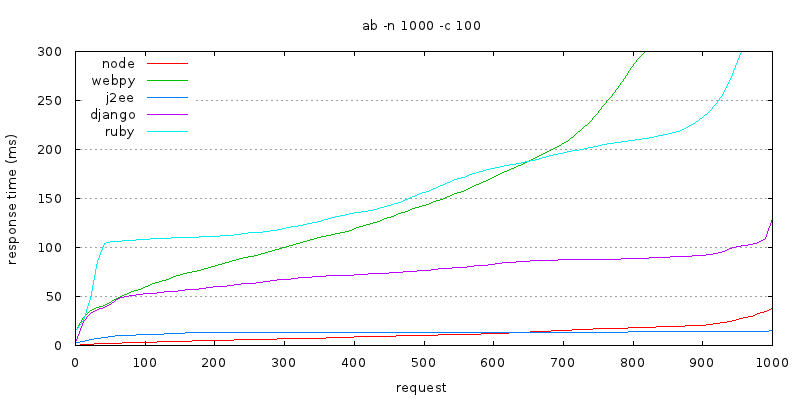
\includegraphics[height=150px]{images/node-bench.png}
\caption{node.js benchmark versus other popular languages/platforms/frameworks}
\label{fig:nodeBench}
\end{figure}

This is not conclusive, since benchmarks can be used only for a particular instance of a program.

The performances were however important because the project is hosted for free and can't demand to too much resources. For this reason, we focused in the most scalable and lightweight solution available: node.js.

\subsubsection{Asynchronous I/O}
\label{sec:async}

The real difference however is the asynchronous I/O and Evented Support (C/C++). Citing ``cloudfoundry.com'' \cite{website:cloudfoundry}: \textit{In order to write a fast and scalable server application, we typically end up writing it in a multi-threaded fashion. While you can build great multi-threaded apps in many languages, it usually requires a lot of expertise to build them correctly. On the other hand, these libraries (along with Chrome’s V8 engine) provide a different architecture that hides the complexities of multi-threaded apps while getting the same or better benefits.}

\textit{Let's compare classic multi-threaded server with an evented, non-blocking I/O server:}

\begin{figure}[H]
\centering % per centrare l'immagine (opzionale)
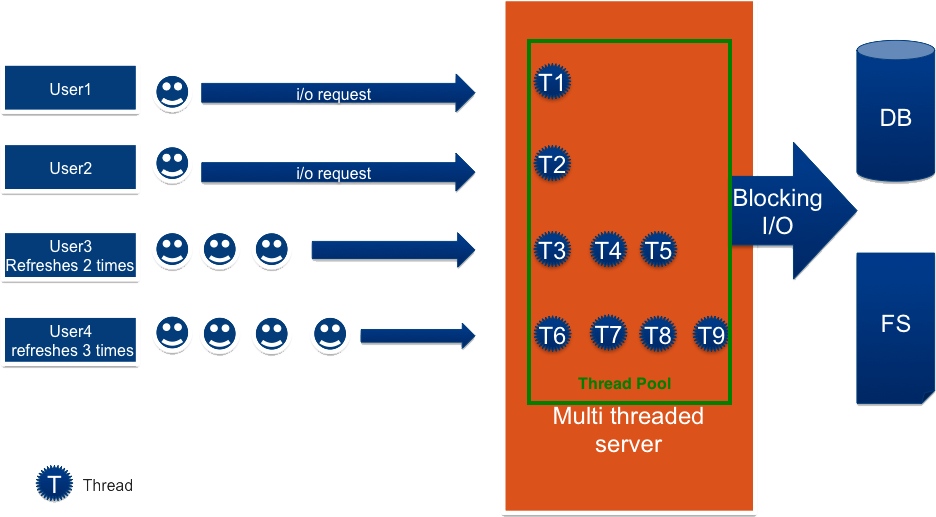
\includegraphics[height=150px]{images/multiThreadedServer.png}
\caption{An example multi-threaded HTTP server using blocking I/O}
\label{fig:multiThreadedServer}
\end{figure}

\textit{The diagram in Figure \ref{fig:multiThreadedServer} depicts a simplified multi-threaded server. There are four users logging into the multi-threaded server. A couple of the users are hitting refresh buttons causing it to use lot of threads. When a request comes in, one of the threads in the thread pool performs that operation, say, a blocking I/O operation. This triggers the OS to perform context switching and run other threads in the thread pool. And after some time, when the I/O is finished, the OS context switches back to the earlier thread to return the result.}

\textit{\textbf{Architecture Summary:} Multi-threaded servers supporting a synchronous, blocking I/O model provide a simpler way of performing I/O. But to handle a heavy load, multi-threaded servers end up using more threads because of the direct association to connections. Supporting more threads causes more memory and higher CPU usage due to more context switching among threads.}

\begin{figure}[H]
\centering % per centrare l'immagine (opzionale)
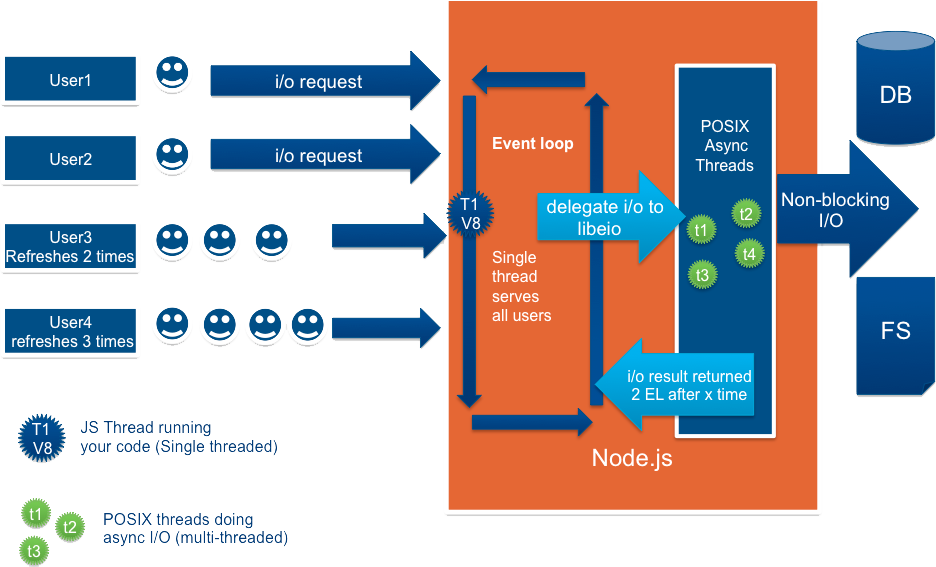
\includegraphics[height=150px]{images/NodeJS-EventedIOAsyncIO_latest.png}
\caption{Event-driven, non-blocking I/O (Node.js server)}
\label{fig:nodejsServer}
\end{figure}

\textit{The diagram in Figure \ref{fig:nodejsServer} depicts how Node.js server works. At a high level, Node.js server has two parts to it:}
\begin{itemize}
\item \textit{At the front, you have Chrome V8 engine (single threaded), event loop and other C/C++ libraries that run your JS code and listen to HTTP/TCP requests;}
\item \textit{And at the back of the server, you have libuv (includes libio) and other C/C++ libraries that provide asynchronous I/O.}
\end{itemize}

\textit{Whenever a request is made from a browser, mobile device, etc., the main thread running in the V8 engine checks if it is an I/O. if it is an I/O then it immediately delegates that to the backside (kernel level) of the server where one of the threads in the POSIX thread pool actually makes async I/O. Because the main thread is now free, it starts accepting new requests/events.}

\textit{And at some point when the response comes back from a database or file system, the backend piece generates an event indicating that we have a result from I/O. And when V8 becomes free from what it is currently doing (remember it is single-threaded), it takes the result and returns it to the client.}

\textit{\textbf{Architecture Summary:} This architecture utilizes an event loop (main thread) at the front and performs asynchronous I/O at the kernel level. By not directly associating connections and threads, this model needs only a main event loop thread and many fewer (kernel) threads to perform I/O. Because there are fewer threads and consequently less context-switching, it uses less memory and also less CPU.}

Another important fact to consider about this choice is also then the easiness of programming in node.js instead of Java. Indeed, node.js is deeply and better connected with the mongoDB NoSQL database, that was perfect for this project and this has effected the whole structure of the program, making it a lot easier and straightforward.

\subsection{Difficulties Node.js}
The main issue with node.js is JavaScript. This language has particular proprieties that are a lot different than what I was used to, in particular Java. I have already program a little in JavaScript, but without using closures, prototypes and asynchronous programming.

The philosophy behind is a lot different, since JavaScript is a weakly object oriented, the opposite of Java. It is also dynamic and has some proprieties of functional languages, for example everything in JavaScript is an object, functions too.

This leads to different design patterns and best practices. Force Java's patters in a JavaScript structure is the wrong way to code in JavaScript.

For this it was really helpful the website \url{http://howtonode.org/} that collects various articles with node.js and JavaScript best practices that help you coding in right way.

Another issue is the continuous change of philosophy. When you are trying to make things work both server-side and client-side you may have to switch continuously from Java to JavaScript and that could make things a bit harder, because the two languages are quite different.

\subsection{Database}

MongoDB (from ``humongous'') is a scalable, high-performance, open source NoSQL database written in C++.

The particularity of MongoDB is that it has a document-oriented storage, in particular it stores BSON documents that are the binary representation of JSON documents.

JSON, acronym for JavaScript Object Notation, has been designed to be as much similar as possible to JavaScript objects. It is now a standard and it is commonly and widely used. So much, that Facebook uses JSON too. in Figure \ref{fig:JSONTrip} you can see how everything in the structure designed simply used JSON Objects. They are managed, changed, stored and got without any conversion from XML, to class-objects, to SQL data or anything similar.

This has a big impact in performace, since MongoDB was designed to be as fast as possible, and to stability, since without any conversion, it is much easier not to have some error in the process.

\begin{figure}[H]
\centering % per centrare l'immagine (opzionale)
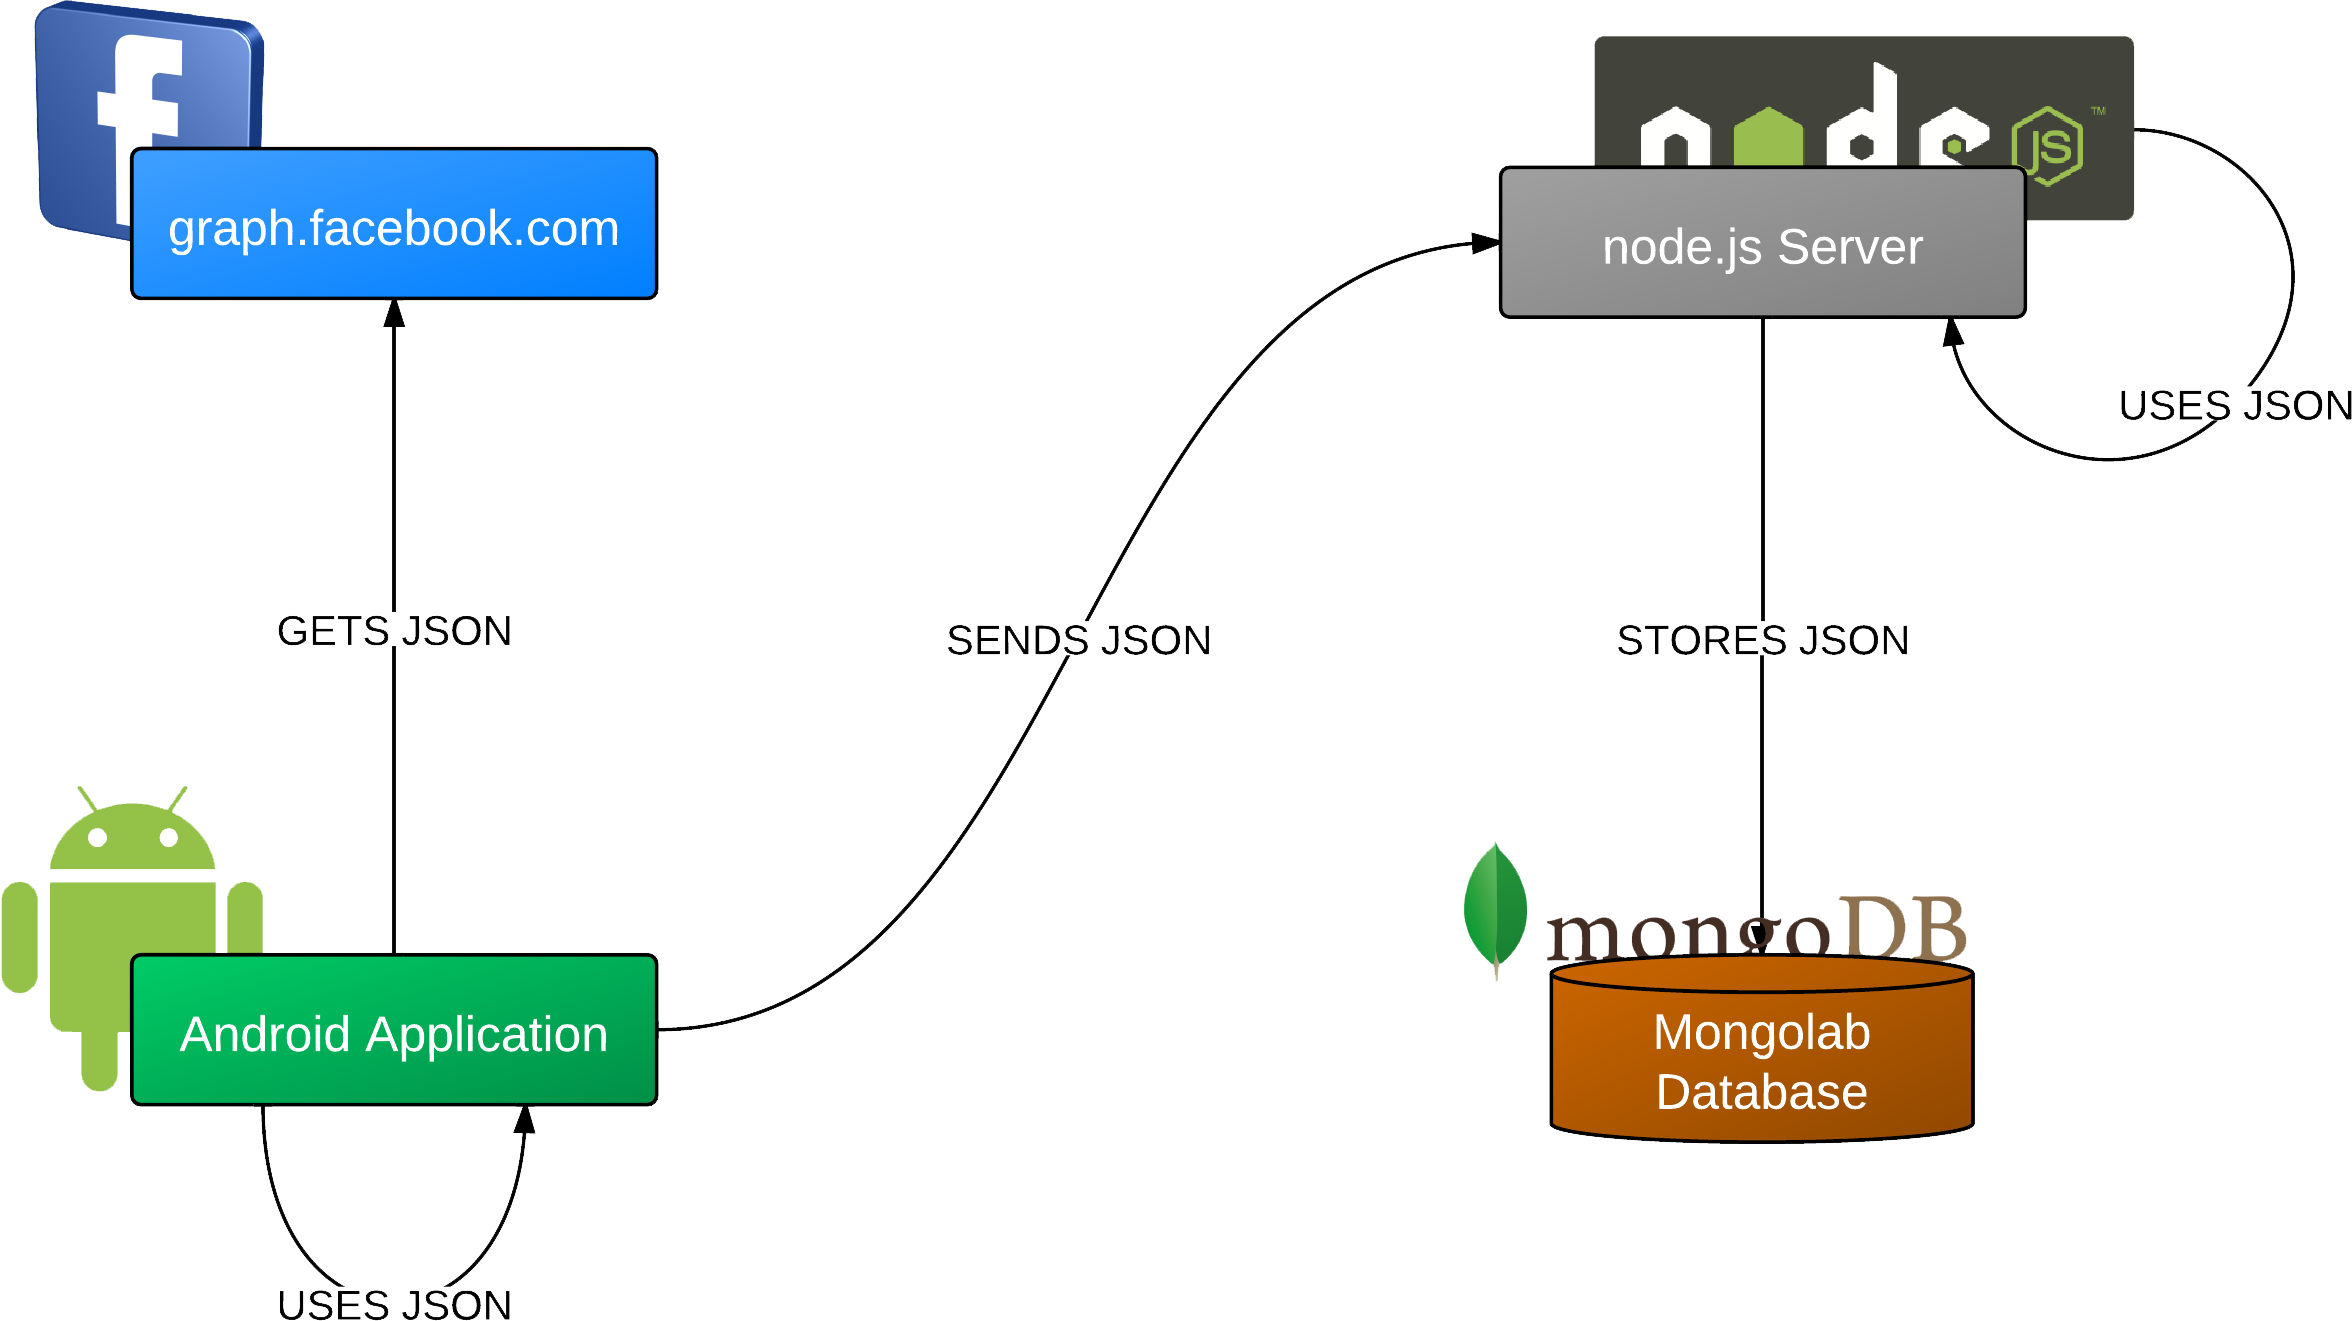
\includegraphics[width=\textwidth]{images/JSONTrip.png}
\caption{How the applications interact with each others, all in JSON}
\label{fig:JSONTrip}
\end{figure}

\subsection{Difficulties with MongoDB \& Mongoose}
I have also dedicated some hours at the study of MongoDB and how to create correctly a database of this type. I was lucky to find the page of the last NoSQL day\footnote{NoSQL day website: \url{http://nosqlday.it/}} with all the speeches given that day. I had a basic knowledge of MongoDB's API but I had no idea of how to model it.

These videos have helped me to create an efficient solution in a quicly way. Solution then I formalized also with the use of Mongoose.

Initially, we used the native driver for MongoDB, not knowing the existence of Mongoose. This was easy to use, but it didn't allows to check if data given are correctly modelled or not. With Mongoose you have this check and you can also set the ``strict'' mode, in order not to insert objects that match the required fields but have also something more than expected.

Furthermore, with MongoDB, the basic rules of E-R modeling, are completely reversed. To cite some meaning considerations about it:

\begin{center}
	\textit{Data duplication and denormalization are first-class citizens.}\cite{website:nosqldatamodeling}
\end{center}

This means that, instead of what happends to E-R databases, the focus is not to avoid duplication or denormalization. So, they are allowed and, in some cases, needed and encouraged. There are some cases where E-R databases aren't the best choice. This is because the E-R system is user and answers oriented, as Ilya Katsov says \cite{website:nosqldatamodeling}:

\begin{itemize}
\item \textit{The end user is often interested in aggregated reporting information, not in separate data items, and SQL pays a lot of attention to this aspect;}
\item \textit{No one can expect human users to explicitly control concurrency, integrity, consistency, or data type validity. That’s why SQL pays a lot of attention to transactional guaranties, schemas, and referential integrity.}
\end{itemize}

\begin{center}
[\dots\unkern]
\end{center}

\textit{NoSQL data modeling often starts from the application-specific queries as opposed to relational modeling:}
\begin{itemize}
\item \textit{Relational modeling is typically driven by the structure of available data. The main design theme is  \textbf{”What answers do I have?”}}
\item \textit{NoSQL data modeling is typically driven by application-specific access patterns, i.e. the types of queries to be supported. The main design theme is \textbf{”What questions do I have?”}}
\end{itemize}

So, as you can see, the focus is not to create a database easily consulted by an human being, but to create a model that can scale easily answering as fast as possible to the questions that the program needs. Although the database structure stays clear, updates and transaction should not be done by hand. For example, in this project the login for a player and an uploader is duplicated. This is because every time you need one of them, you shouldn't download two tables but only one.

As Gabriele Lana says \cite{website:mongodbwithstyle}:

\begin{center}
	\textit{The best design is the one where needed data can be easily extracted}
\end{center}

\begin{center}
	\textit{The way you need to query your data should influence your design}
\end{center}

\begin{figure}[H]
\centering % per centrare l'immagine (opzionale)
\includegraphics[width=\textwidth]{images/mongodbwithstyleafter.png}
\caption{MongoDB performance analysis of the queries}
\label{fig:mongodbwithstyle}
\end{figure}

In Figure \ref{fig:mongodbwithstyle} you can see how you can tune your queries with MongoDB. With this, you can ask the engine to explain how it processes the query, if indexes are being used and how much time is needed to answer the request. You can also set the engine so to log every request that is slower than a given time, to find the queries bad formed, fix them and speed up your application.

\newpage

\section{Actual application}
\label{sec:actualApplication}

In this Section we will see the finished application and how the requirements have been satisfied. Every requirement has been tracked, so the comparison can be done easily.  

\subsubsection{Mobile Application (UC\_1)}

Most of the requirements of the UC\_1 are in the home screen in Figure \ref{fig:homescreen}. The settings are in Figure \ref{fig:singlePlayer}. Before entering the home screen, the user sees the EULA, as you can see in Figure \ref{fig:eulaScreen} and then an explanation of how to play, Figure \ref{fig:howToPlay}.

\begin{figure}[H]
        \begin{subfigure}[b]{0.3\textwidth}
                \centering
\includegraphics[width=100px]{images/screenshot/mobile/eulaScreen.png}
\caption{EULA screen}
\label{fig:eulaScreen}
        \end{subfigure}%
        ~ %add desired spacing between images, e. g. ~, \quad, \qquad etc. 
          %(or a blank line to force the subfigure onto a new line)
        \begin{subfigure}[b]{0.3\textwidth}
                \centering
\includegraphics[width=100px]{images/screenshot/mobile/homescreen.png}
\caption{Home screen}
\label{fig:homescreen}
        \end{subfigure}
        ~ %add desired spacing between images, e. g. ~, \quad, \qquad etc. 
          %(or a blank line to force the subfigure onto a new line)
        \begin{subfigure}[b]{0.3\textwidth}
                \centering
\includegraphics[width=100px]{images/screenshot/mobile/howToPlayScreen.png}
\caption{How to play screen}
\label{fig:howToPlay}
        \end{subfigure}
        \caption{The Main screens}
        \label{fig:mainScreens}
\end{figure}

\textbf{Status:}  70\%.
		\begin{description}
			\item[UC\_1.1:] [necessary] \textbf{100\%.} The login is allowed by the Facebook system that tracks user's informations. The system has been set to allow also the addition of further methods;
			\item[UC\_1.2:] [optional] \textbf{100\%} The Wizard has changed with only a simple screen showing how to use the program the first time that the user opens the application, as you can see in Figure \ref{fig:howToPlay}. There is no need of further explanations;
			\item[UC\_1.3:] [optional] \textbf{100\%} The Social  (section \ref{sec:social}) has been done a little differently than what expected. Since the loss of the Wizard buttons, we decided to split the social into ``rate the application'' and everything else, to make things easier. Both are completely done and ready;
			\item[UC\_1.4:] [desirable] \textbf{50\%} The Settings  (section \ref{sec:settingsActualApplication}) are prepared but not used, since there aren't needed yet;
			\item[UC\_1.5:] [desirable] \textbf{0\%} We hoped that the ranking would be easily handled by one of the SDK available. Instead, there is not easy way to do it, you have to completely merge your application with the SDK given and only in some cases you have access to the web API. Papaya Mobile was the best solution but you have to rewrite the application completely using their SDK if you want to enter in their network;
			\item[UC\_1.6:] [necessary] \textbf{80\%} The Single Player (section \ref{sec:singlePlayer}) is almost completely done. We have deleted the option to show the screenshot, since it is not the focus of the project and the 50\% 50\%, but the rest of the functionalities are fully working. The report of the track, although planned and prepared server-side, it is not working yet (since the C2C solution isn't already available);
			\item[UC\_1.7:] [optional] \textbf{0\%} The Multiplayer was included in future prospective, but we have already stated that was really unlikely to complete that in time;
			\item[UC\_1.8:] [optional] \textbf{70\%} Download the tracks. The users may want to play also off-line. This option has already been planned and prepared server side. The only thing needed is the storage of the quests in a persistent way and not only temporary when playing.
		\end{description}

\subsubsection{Social (UC\_1.3)}
\textbf{Status: 100\%.} The rate of the application has been implemented with a button separated with the rest of the others requirements. The others are implemented with a screen where the user can choice his preferred system to share the application, that must be installed in the device by the user. So, the feature available can be less or even more, according to what the user has installed on the device. You can see a screenshot of this feature in Figure \ref{fig:shareGufy}.

\begin{figure}[H]
\centering % per centrare l'immagine (opzionale)
\includegraphics[width=200px]{images/shareScreen.png}
\caption{How the use case has been implemented}
\label{fig:shareGufy}
\end{figure}

\subsubsection{Settings (UC\_1.4)}
\label{sec:settingsActualApplication}

The settings have been changed. The change of language is no longer needed since the program can automatically detect the language of the device. The categories and the user statistics aren't now ready. So, in Figure \ref{fig:settings}, you can see the settings fully working, but without redirecting to something more than the Facebook login and the Single Player.

\begin{figure}[H]
\centering % per centrare l'immagine (opzionale)
\includegraphics[width=150px]{images/screenshot/mobile/settings.png}
\caption{Settings screen}
\label{fig:settings}
\end{figure}

\textbf{Status:} 50\%
		\begin{description}
			\item[UC\_1.4.1:] [necessary] \textbf{100\%.} The change of language is automatic and is based on the language of the device. The languages available are curretly italian and english as required;
			\item[UC\_1.4.2:] [desirable] \textbf{20\%} Categories are ready server-side and the data is already given to the device that, however, can't handle them right now;
			\item[UC\_1.4.3:] [desirable] \textbf{50\%} The log-out in Facebook is already implemented but since the settings screen is not already available, it cannot be used right now;
			\item[UC\_1.4.4:] [optional] \textbf{20\%} The user's statistics are currently logged by the server but not handled and used by the device.
		\end{description}

\subsubsection{Single Player (UC\_1.6)}

In the Figure \ref{fig:downloadingScreen} we can see the screen that the user will see when she starts playing. This screen is avoided if the ``How To Play Screen'', Figure \ref{fig:howToPlay}, is shown and in every following turn of the game. In Figure \ref{fig:singlePlayerMainScreen} you can se what appears when the user clicks on the play button. We have choosen to do so, to avoid for the user to process a lot of informations that she can't use before clicking on play. The Figure \ref{fig:singlePlayerEndTrack} shows the replay button and the Figure \ref{fig:singlePlayerSkippedTrack} shows what happens if the user clicks on ``skip'' button or chooses an answer. The image shown is usually a funny picture, since as we have seen in Section \ref{sec:personae}, our players are typically young and this may make the game more engaging.

\begin{figure}[H]
        \begin{subfigure}[b]{0.5\textwidth}
                \centering
\includegraphics[width=150px]{images/screenshot/mobile/SinglePlayerLoading.png}
\caption{The downloading of the quests screen}
\label{fig:downloadingScreen}
        \end{subfigure}%
        ~ %add desired spacing between images, e. g. ~, \quad, \qquad etc. 
          %(or a blank line to force the subfigure onto a new line)
        \begin{subfigure}[b]{0.5\textwidth}
                \centering
\includegraphics[width=150px]{images/screenshot/mobile/SinglePlayerPlaying.png}
\caption{The single player start screen}
\label{fig:singlePlayerMainScreen}
        \end{subfigure}
        ~ %add desired spacing between images, e. g. ~, \quad, \qquad etc. 
          %(or a blank line to force the subfigure onto a new line)
        \begin{subfigure}[b]{0.5\textwidth}
                \centering
\includegraphics[width=150px]{images/screenshot/mobile/SinglePlayerBeforeStart.png}
\caption{The single player when a track is ended}
\label{fig:singlePlayerEndTrack}
        \end{subfigure} 
        ~ %add desired spacing between images, e. g. ~, \quad, \qquad etc. 
          %(or a blank line to force the subfigure onto a new line)
        \begin{subfigure}[b]{0.5\textwidth}
                \centering
\includegraphics[width=150px]{images/screenshot/mobile/SinglePlayerSkip.png}
\caption{The single player when a track is skipped}
\label{fig:singlePlayerSkippedTrack}
        \end{subfigure}
        \caption{The Single Player screens}
        \label{fig:singlePlayer}
\end{figure}

	\textbf{Status:} 80\%
		\begin{description}
			\item[UC\_1.6.1:] [necessary] \textbf{100\%.}  Listen/stop the movie track is completely working;
			\item[UC\_1.6.2:] [optional] \textbf{0\%.} To see a screenshot it is not strictly needed and it is difficult to position in the screen, so it hasn't been implemented yet;
			\item[UC\_1.6.3:] [necessary] \textbf{100\%} The ability to guess the movie is obviously necessary and has been implemented successufully;
			\item[UC\_1.6.4:] [necessary] \textbf{100\%} The user can skip the tracks 3 times, as you can see in Figure \ref{fig:singlePlayerSkippedTrack};
			\item[UC\_1.6.5:] [desirable] \textbf{40\%} The report of the track has been implemented only server-side, it is still not available since it should come with the C2C feature;
			\item[UC\_1.6.6:] [optional] \textbf{100\%} The 50\% \& 50\% has been created;
			\item[UC\_1.6.7:] [desirable] \textbf{100\%} The listen again is integrated with functionality UC\_1.6.1 as you can see in Figure \ref{fig:singlePlayerEndTrack}.
		\end{description}

\subsection{Game Site (UC\_2)}
\label{sec:gameSiteActualSite}
In this Section we will describe how the website has been developed. You can see Figure \ref{fig:siteIndex} where is shown the index of the main page. In it there is a slider built upon a phone, in order to show the application as it would be something real. In Figure \ref{fig:siteContactForm} you can see the contact form where the user can send us a feedback. In Figure \ref{fig:siteAbout} there is the about page, where we explain the Project and our role in it. In Figure \ref{fig:siteLogin} you can see how we manage now the human login to the website and in Figure \ref{fig:siteUpload} and Figure \ref{fig:siteUploadDonePage} you see how we handle the upload of the tracks.

\begin{figure}[H]
        \begin{subfigure}[b]{\textwidth}
                \centering
\includegraphics[width=\textwidth]{images/screenshot/site/index.png}
\caption{The index of the website}
\label{fig:siteIndex}
        \end{subfigure}%
\end{figure}
\begin{figure}[H]   
        %add desired spacing between images, e. g. ~, \quad, \qquad etc. 
          %(or a blank line to force the subfigure onto a new line)
        \begin{subfigure}[b]{\textwidth}
                \centering
\includegraphics[width=\textwidth]{images/screenshot/site/index-contact.png}
\caption{The contact form of the website}
\label{fig:siteContactForm}
        \end{subfigure}     
        
        %add desired spacing between images, e. g. ~, \quad, \qquad etc. 
          %(or a blank line to force the subfigure onto a new line)
        \begin{subfigure}[b]{\textwidth}
                \centering
\includegraphics[width=\textwidth]{images/screenshot/site/about.png}
\caption{The about page}
\label{fig:siteAbout}
        \end{subfigure} 
\end{figure}
\begin{figure}[H]   
         %add desired spacing between images, e. g. ~, \quad, \qquad etc. 
          %(or a blank line to force the subfigure onto a new line)
        \begin{subfigure}[b]{\textwidth}
                \centering
\includegraphics[width=\textwidth]{images/screenshot/site/login.png}
\caption{The login page}
\label{fig:siteLogin}
        \end{subfigure}
        \caption{The Game Site screens}
        \label{fig:gameSite}
\end{figure}

\textbf{Status:} 80\%
		\begin{description}
			\item[UC\_2.1:] [necessary] \textbf{100\%.} The login/signin is now available as a custom solution for users and with facebook for mobile people, as you can see in Figure \ref{fig:siteLogin}. The login with facebook is restricted to mobile only because the first users to access the website are only people allowed by us;
			\item[UC\_2.2:] [desiderable] \textbf{100\%} The wizard has been done using a slider that shows the screenshots of the application like they were on an actual Android device, as you can see in Figure \ref{fig:siteIndex};
			\item[UC\_2.3:] [optional] \textbf{100\%} The social connection has been done easily using add-on already built by Facebook and Twitter, as you can see in Figure \ref{fig:siteContactForm};
			\item[UC\_2.4:] [desirable] \textbf{0\%} The ranking, as already explained, has not been already done;
			\item[UC\_2.5:] [necessary] \textbf{100\%} The project info has been handled with an about page regarding the projects and team members, the one shown in Figure \ref{fig:siteAbout};
			\item[UC\_2.6:] [necessary] \textbf{100\%} You can see the contact form in Figure \ref{fig:siteContactForm};
			\item[UC\_2.7:] [necessary] \textbf{100\%} As already said, the language change is built-it in the Android system;
			\item[UC\_2.8:] [desirable/optional] \textbf{20\%} Only the uploading is now available, as you can see in Figure \ref{fig:siteUpload} and Figure \ref{fig:siteUploadDonePage};
			\item[UC\_2.9:] [necessary] \textbf{80\%} all the Game API necessary functionalities have been implemented. For a detailed description, see Section \ref{sec:GameApiFinal}.
		\end{description}
	
\subsubsection{Quest Management (UC\_2.8)}

In this section we will describe how the Quest Management system have been implemented. Since the C2C feature has only been planned, it is basically only the uploading page, seen in Figure \ref{fig:siteUpload} and Figure \ref{fig:siteUploadDonePage}.

\begin{figure}[H]    
         %add desired spacing between images, e. g. ~, \quad, \qquad etc. 
          %(or a blank line to force the subfigure onto a new line)
        \begin{subfigure}[b]{\textwidth}
                \centering
\includegraphics[width=\textwidth]{images/screenshot/site/upload.png}
\caption{The upload page}
\label{fig:siteUpload}
        \end{subfigure}
        
        %add desired spacing between images, e. g. ~, \quad, \qquad etc. 
          %(or a blank line to force the subfigure onto a new line)
        \begin{subfigure}[b]{\textwidth}
                \centering
\includegraphics[width=\textwidth]{images/screenshot/site/uploadDone.png}
\caption{The upload result page}
\label{fig:siteUploadDonePage}
        \end{subfigure}
\end{figure}

\textbf{Status:} 20\%
		\begin{description}
			\item[UC\_2.8.1:] [necessary] \textbf{100\%.} The uploading feature is already full available;
			\item[UC\_2.8.2:] [optional] \textbf{0\%}. The deletion of a quest is not available now from the website;
			\item[UC\_2.8.3:] [optional] \textbf{0\%}. Once a quest is uploaded, it cannot be changed right now;
			\item[UC\_2.8.4:] [optional] \textbf{0\%}. The comments aren't enabled yet;
			\item[UC\_2.8.5:] [optional] \textbf{0\%}. The quests rating isn't available;
			\item[UC\_2.8.6:] [optional] \textbf{0\%}. The deletion of a track can be done only with the database access.
		\end{description}

\subsubsection{Game API (UC\_2.9)}
\label{sec:GameApiFinal}

In this Section we will describe the APIs that have been actually done. It is not something visible, since they are only JSON responses for the mobile application.

\textbf{Status:} 95\%
		\begin{description}
			\item[UC\_2.9.1:] [necessary] \textbf{100\%.} The add of a new user has been done automatically with the Facebook login;
			\item[UC\_2.9.2:] [necessary] \textbf{100\%}. It is possible to get the user data with a simple request;
			\item[UC\_2.9.3:] [desirable] \textbf{100\%}. It is already possible to download the database, but only server-side;
			\item[UC\_2.9.4:] [desirable] \textbf{60\%}. The ranking data are stored and you can get them for a single user;
			\item[UC\_2.9.5:] [necessary] \textbf{100\%}. The download of the quest is ready;
			\item[UC\_2.9.6:] [necessary] \textbf{100\%}. The points are already handled.
		\end{description}

\subsection{Result Analysis}
\subsubsection{Tracks management}

\begin{figure}[H]   
         %add desired spacing between images, e. g. ~, \quad, \qquad etc. 
          %(or a blank line to force the subfigure onto a new line)
        \begin{subfigure}[b]{\textwidth}
                \centering
\includegraphics[width=\textwidth]{images/accelerometerXPatterns1.png}
\caption{The first subject - X values of the accelerometer}
\label{fig:firstSubjectPatterns}
        \end{subfigure}

         %add desired spacing between images, e. g. ~, \quad, \qquad etc. 
          %(or a blank line to force the subfigure onto a new line)
        \begin{subfigure}[b]{\textwidth}
                \centering
\includegraphics[width=\textwidth]{images/accelerometerXPatterns2.png}
\caption{The second subject}
\label{fig:secondSubjectPatterns}
        \end{subfigure}
        \caption{Two patterns analysed with the application - X values of the accelerometer}
        \label{fig:secondSubjectPatterns}
\end{figure}

This requirement cannot be seen with screenshot, but only with the diagrams seen in Section \ref{sec:planningGameSite}. However, you can see in Figure the data processed after that they have been collected. The tracks are really similar also at naked eye.

\textbf{status:} 100\% these requirements is fully implemented and ready to be used.

\subsubsection{DTW}
The DTW algorithms are ready to be used. They are based on the algorithms used by the MHYAM Project \cite{MHYAM}, but have been moved server side.

\textbf{status:} 100\% this requirement is fully implemented and ready to be used.

\subsubsection{Oracle}
You can see in Figure \ref{fig:oracle} the application used as reference for the tests. The results where the same with the How To Play screen, Figure \ref{fig:howToPlay}, but we wonder what would succeed in real world and after some time that the screen doesn't show up.

\begin{figure}[H]
\centering % per centrare l'immagine (opzionale)
\includegraphics[width=150px]{images/screenshot/mobile/oracle.png}
\caption{The oracle application}
\label{fig:oracle}
\end{figure}

\textbf{status:} 100\%, it was asked to hack the Android phone system to add this feature only for rooted device. For testing purposes was rewritten the basic application and that would be used for these monitored tests, since the results are similar.

\subsubsection{Cluster analysis}

\textbf{status:} 40\%, this type of analysis has already been tested with the Orange tool and Wikipedia's data. However, we need actual data to perform this analysis and some hours to do it in an accurate way.

\subsection{Requirements (UC\_4)}
We now see how we handled the requirements showed in Section \ref{sec:requirements}.

\subsubsection{RQ\_4.1 - encryption}
The encryption was successfully implemented using the AES at 128 bit encryption, avoiding for the user to know and manipulate the data sent to the server.
\subsubsection{RQ\_4.2 - privacy solution}
The privacy solution was accomplished in the way you can see in Figure \ref{fig:securitySystem}. The Android application sends the data to the server in two independent steps.
		\begin{itemize}
			\item The first is the data send for the analysis. This is handled by an external library, based on the application by Earlence Fernandes, rewritten and adapted by me. It uses an hash based on the id and the birthday (that is required for the facebook account, so there is always a date) to create an unique id;
			\item To the player collection is sent only the year and not the whole date, with also some more data about the user.
		\end{itemize}

\begin{figure}[H]
\centering % per centrare l'immagine (opzionale)
\includegraphics[width=\textwidth]{images/sendInfoToServer.png}
\caption{Security system to preserve the privacy of the users}
\label{fig:securitySystem}
\end{figure}

\subsubsection{RQ\_4.3 - GUI}
The GUI is really simple. So simple that there is no need of a manual or a guided tour to explain the features of the application. The GUI attractiveness is not something that can be measured, we have tried to create a clean GUI, although I'm not a designer.
\subsubsection{RQ\_4.4 - movies' size}
The movies length has been limited in size when the user uploads the file.
\subsubsection{RQ\_4.5 - play his movies}
The movies are uploaded by the administrator, so this requirement has a sense only if the C2C solution is opened and available, but is not.
\subsubsection{RQ\_4.6 - skips}
Requirement done successfully, as you have already seen in Figure \ref{fig:singlePlayerSkippedTrack}.
\subsubsection{RQ\_4.7 - hardness of a movie}
Initially, this requirement has no meaning but it has been already implemented. The fact is that initially all the movies start from the same point. It is needed some time of learning before the server can divide the movies in different levels and in this time, is meaningless to make some distinctions, because all the tracks will be at medium level. So all the statistics will be record from the very first time, but this future will be available only later.

\newpage

\section{Validation}
\label{sec:validation}

To ensure an high code's quality we have used different metrics that have helped us to write better code avoiding bad practices, bad coding or bad planning that can automatically find out.

%Furthermore, we have automated some the main tests for the website.

\subsection{Android}

In this Section we will analyse how we have validate the quality of the Android application. Every tests and metrics have been done using Eclipse and two actual devices: a HTC Desire HD and a LG Optimus Me.

\subsubsection{Lint}
To assure that the code's quality stays high, we have decided to use the automatically lint-helper embedded with the Android Plugin for the Eclipse IDE.

This plugin allows you to check:

\begin{itemize}
\item Missing translations (and unused translations);
\item Layout performance problems (all the issues the old layoutopt tool used to find, and more);
\item Unused resources;
\item Inconsistent array sizes (when arrays are defined in multiple configurations);
\item Accessibility and internationalization problems (hardcoded strings, missing contentDescription, etc);
\item Icon problems (like missing densities, duplicate icons, wrong sizes, etc);
\item Usability problems (like not specifying an input type on a text field);
\item Manifest errors.
\end{itemize}

This allows you to delete useless code and fix little and medium problems regarding your code.

\subsubsection{Eclipse Metrics}

This plugin has a wide range of metrics and tools to judge code's quality. With it you can analyse different aspect of your code and the great advantage is that it can automatically warn you when there is something wrong, directly in the IDE.

The results were a code of good quality, also because we followed the Java official conventions \cite{website:javacodeconventions}.

Let's see now our code's statistics.

\begin{figure}[H]
\centering % per centrare l'immagine (opzionale)
\includegraphics[width=300px]{images/codequality/cyclomatic_complexity.png}
\caption{Cyclomatic complexity of the code}
\label{fig:cyclomaticComplexity}
\end{figure}

In Figure \ref{fig:cyclomaticComplexity} we can see the Cyclomatic Complexity of the code. As we can see, the results are even better than expected and only a few methods has a complexity superior than 5.

\textit{This metric is an indication of the number of 'linear' segments in a method (i.e sections of code with no branches) and therefore can be used to determine the number of tests required to obtain complete coverage. It can also be used to indicate the psychological complexity of a method.}\cite{website:eclipse-metrics}

\begin{figure}[H]
\centering % per centrare l'immagine (opzionale)
\includegraphics[width=300px]{images/codequality/feature_envy.png}
\caption{Feature envy}
\label{fig:featureEnvy}
\end{figure}

In Figure \ref{fig:featureEnvy} we can see the level of Feature Envy that there is the code. The result is really good, since the classes are well divided and this level is really low. The only few methods that has an higher values are the ones dedicated to initialize important services or activities, methods not so easy to split.

\textit{Feature Envy occurs when a method is more interested in the features (methods and fields) of other classes than its own. The solution if it exists at all, is straightforward; move the method to the class that it is most envious of, passing any parameters the new method requires. If only part of the method demonstrates this envy, extract that part and then move the new method into the envied class. Sometimes this is not possible, since the envied class may be available only in a non-modifiable form.}\cite{website:eclipse-metrics}\cite{website:eclipse-metrics}

\begin{figure}[H]
\centering % per centrare l'immagine (opzionale)
\includegraphics[width=300px]{images/codequality/lines_of_code_in_methods.png}
\caption{Lines of code in methods}
\label{fig:linesOfCode}
\end{figure}

In Figure \ref{fig:linesOfCode} we can see the length of the methods used in the classes. This parameter is good too, since the big number of methods in the code. The focus was indeed to isolate the functions of every piece of code in well defined methods and classes.

\begin{figure}[H]
\centering % per centrare l'immagine (opzionale)
\includegraphics[width=300px]{images/codequality/number_of_levels.png}
\caption{Number of levels}
\label{fig:numberOfLevels}
\end{figure}

In Figure \ref{fig:numberOfLevels} we can see the number of levels that are done in the code. This metric shows no methods out of the bounds. The focus indeed was to keep the code simple and straightforward.

\textit{This metric is an indication of the maximum number of levels of nesting in a method. The idea of the metric is that a large Number Of Levels increases complexity and reduces comprehensibility. In addition, such methods generally (but not necessarily) operate at the lowest level of abstraction or at mixed levels of abstraction, both of which contribute to the confusion.}\cite{website:eclipse-metrics}

\begin{figure}[H]
\centering % per centrare l'immagine (opzionale)
\includegraphics[width=300px]{images/codequality/number_of_parameters.png}
\caption{Number of parameters}
\label{fig:numberOfParameters}
\end{figure}

In Figure \ref{fig:numberOfParameters} we can see the number of parameters given to the functions. The outcomes are really good, since every method has less than 4 parameters. This leads to a good class separation.

\begin{figure}[H]
\centering % per centrare l'immagine (opzionale)
\includegraphics[width=300px]{images/codequality/number_of_statements.png}
\caption{Number of statements}
\label{fig:numberOfStatements}
\end{figure}

In Figure \ref{fig:numberOfStatements} we can see the number of statements. This measure is different than the number of code's lines, since in one line can be more than one sentence. As in the previous diagram, also this result in very good.

\begin{figure}[H]
\centering % per centrare l'immagine (opzionale)
\includegraphics[width=300px]{images/codequality/numbers_of_locals_in_scope.png}
\caption{Number of locals in scope}
\label{fig:numberOfLocalsInScope}
\end{figure}

In Figure \ref{fig:numberOfLocalsInScope} we can see that this metric is almost never out of bounds.

\textit{This metric is an indication of the maximum number of local variables in scope at any point in a method. The idea of the metric is that a large Number Of Locals In Scope increases complexity and reduces comprehensibility.}\cite{website:eclipse-metrics}

\subsection{Game Site}

The Game Site, published with the domain: \url{http://gufy.filnik.com/}, has different metrics that defines its quality.

\subsubsection{HTML and site appearance}

First of all, the HTML mark-up should validate correctly. This has been done with the W3C validator\footnote{W3C validator: \url{http://validator.w3.org/}} for every page, that now validates correctly.

Then, we tested the website with different browsers. We used:

\begin{itemize}
\item Google Chrome, version 21.0.1180.89 on Mac OS X 10.7 Lion;
\item Mozilla Firefox, version 15 on Mac OS X 10.7 Lion;
\item Safari, version 6.0 on Mac OS X 10.7 Lion;
\item Internet Explorer 7, emulated with a web service;
\item Dolphin Browser HD, version 8.7.0, on an HTC Desire HD.
\end{itemize}

All these browsers rendered correctly the website as expected. The site is simple, so we don't have major usability or accessibility issues.

\subsubsection{node.js}

The client-side JavaScript used until now is really few. No more than 100 lines of code. For this reason it is meaningless speak of code quality for it.

Regarding instead the server-side JavaScript used, the amount of code is instead significant. However, here too the amount of code is not that much. Indeed, we are speaking of around 1000 lines of code.

For this reason, the main file: \texttt{server.js} haven't been split in different classes that wouldn't have been bigger than 50 lines of code, fragmenting the application in different and unusable files.

This makes it also easier to be checked. Using the Sublime Text is possible to check automatically the code's quality using the \url{http://www.jshint.com/} utility in an easy way.

This allows you to check:
\begin{itemize}
\item unsafe for..in;
\item empty blocks;
\item unsafe comparisons;
\item assignments inside if/for/...;
\item functions inside loops;
\item the use of eval;
\item unsafe line breaks;
\item the use of bitwise operators;
\item code is not in strict mode;
\item undefined variables;
\item variables defined but not used;
\item when blocks omit {};
\item when new is used for side effects.
\end{itemize}

Furthermore, the code has been set in strict mode, so it must be of higher quality just to compile.

For a better analysis, we used JSMeter \cite{website:jsmeter}. This allows us to see if the code is mature for the release or not.

% Table generated by Excel2LaTeX from sheet 'Sheet1'
\noindent \begin{tabular}{|l|p{56px}|l|l|l|l|l|l|l|l|l|l|}
\hline
{\bf Ln} & {\bf Function} & {\bf St} & {\bf Ln} & {\bf Cm} & {\bf Cm\%} & {\bf B} & {\bf D} & {\bf C} & {\bf HV} & {\bf HP} & {\bf PL} \\
\hline
         1 &   [[code]] &        432 &        513 &         28 &     5.46\% &          0 &          0 &          1 &       1770 &       4.75 &    0.00268 \\
\hline
        48 &        log &         14 &         10 &          0 &        0\% &          0 &          0 &          1 &        185 &       8.00 &     0.0432 \\
\hline
        49 & log. getErrorObject &          7 &          2 &          0 &        0\% &          1 &          0 &          3 &       32.3 &       4.75 &      0.147 \\
\hline
        72 & (An1) &         17 &         24 &          6 &       25\% &          0 &          0 &          1 &        415 &       4.75 &     0.0114 \\
\hline
        88 & (An1).(A1) &          1 &          4 &          2 &       50\% &          0 &          0 &          1 &       8.42 &       4.75 &      0.564 \\
\hline
        93 & (An1).(An2) &          1 &          3 &          1 &    33.33\% &          0 &          0 &          1 &       8.42 &       4.75 &      0.564 \\
\hline
        99 & initDb &          5 &          5 &          0 &        0\% &          0 &          0 &          1 &       83.4 &       4.75 &     0.0570 \\
\hline
       100 & initDb. (An1) &          1 &          2 &          0 &        0\% &          0 &          0 &          1 &       8.42 &       4.75 &      0.564 \\
\hline
       109 & randXToY &          3 &          4 &          0 &        0\% &          1 &          0 &          3 &        111 &       15.5 &      0.140 \\
\hline
       115 & rmOldest &         16 &         14 &          0 &        0\% &          3 &          3 &          4 &        228 &       11.6 &     0.0509 \\
\hline
       134 & randQuest &         19 &         17 &          0 &        0\% &          5 &          1 &          9 &        326 &       15.5 &     0.0475 \\
\hline
       153 & basic\_login &         10 &         21 &          0 &        0\% &          3 &          1 &          4 &        303 &       15.5 &     0.0512 \\
\hline
       176 & display404 &          9 &         22 &          0 &        0\% &          0 &          0 &          1 &        557 &       11.6 &     0.0208 \\
       \hline
       200 &    generic &         11 &         12 &          1 &     8.33\% &          2 &          1 &          3 &        187 &       15.5 &     0.0829 \\
\hline
       215 & (An2) &          3 &          2 &          0 &        0\% &          0 &          0 &          1 &       15.8 &       11.6 &      0.734 \\
\hline
       219 & (An3) &         21 &         15 &          0 &        0\% &          2 &          1 &          6 &        290 &       11.6 &     0.0400 \\
\hline
       224 & (An3). callback &          3 &          1 &          0 &        0\% &          0 &          0 &          1 &       15.8 &       8.00 &      0.506 \\
\hline
       236 & (An4) &         21 &         23 &          1 &     4.35\% &          1 &          1 &          2 &        181 &       11.6 &     0.0641 \\
\hline
       240 & (An4).(An1) &         11 &         15 &          1 &     6.67\% &          1 &          2 &          2 &        215 &       8.00 &     0.0372 \\
\hline
       262 & (An5) &         44 &         68 &          6 &     8.82\% &          2 &          2 &          3 &        351 &       11.6 &     0.0330 \\
\hline
       270 & (An5). outputFunction &          2 &          4 &          0 &        0\% &          0 &          0 &          1 &       97.7 &       8.00 &     0.0819 \\
\hline
       295 & (An5).(An1) &         22 &         35 &          3 &     8.57\% &          0 &          2 &          1 &        226 &       11.6 &     0.0513 \\
\hline
       311 & (An5).(An1). (An1) &         13 &         19 &          2 &    10.53\% &          2 &          4 &          3 &        336 &       8.00 &     0.0238 \\
\hline
       335 & (An6) &         79 &         70 &          0 &        0\% &          2 &          1 &          4 &        448 &       11.6 &     0.0259 \\
\hline
       359 & (An6).(An1) &         53 &         46 &          0 &        0\% &          3 &          3 &          6 &       1010 &       11.6 &     0.0115 \\
\hline
       398 & (An6).(An1). (An1) &          4 &          4 &          0 &        0\% &          1 &          2 &          2 &       25.4 &       11.6 &      0.457 \\
\hline
       411 & (An7) &         46 &         47 &          0 &        0\% &          2 &          1 &          4 &        453 &       11.6 &     0.0256 \\
\hline
       436 & (An7).(An1) &         20 &         17 &          0 &        0\% &          1 &          2 &          2 &        185 &       8.00 &     0.0432 \\
\hline
       447 & (An7).(An1). (An1) &          5 &          6 &          0 &        0\% &          1 &          3 &          2 &       43.0 &       11.6 &      0.270 \\
\hline
       461 & (An8) &         21 &         36 &          8 &    22.22\% &          1 &          1 &          2 &        357 &       11.6 &     0.0325 \\
\hline
       500 & (An9) &          3 &          3 &          0 &        0\% &          0 &          0 &          1 &       35.8 &       4.75 &      0.133 \\
\hline
       505 & (An10) &          3 &          3 &          1 &    33.33\% &          0 &          0 &          1 &       31.1 &       11.6 &      0.373 \\
\hline
       509 & (An11) &          3 &          1 &          0 &        0\% &          0 &          0 &          1 &       15.8 &       11.6 &      0.734 \\
\hline
\end{tabular}
\vspace{10px}

For this analysis we will take a look only on \texttt{server.js} file, since there is the most important part of the code. The table shows:
\begin{enumerate}
\item line where every function begins in the main file;
\item function name;
\item number of sentences for every method. We can see that it is not so good as in the Android part. The focus in node.js was to keep everything in the same place and, not to complicate too much the code, it hasn't been divided in a lot of small functions, as in Java;
\item lines of code;
\item number of comments. This column shows how  few are the comments right now. The mainly two: the first is for the duplication. I write usually variables whose name is really clear and divide the code in blocks with meaningful names. In this way, comments are useless and can lead to duplication of informations. The second on is that I am developing the project alone and I don't need to explain to myself what my code does. When it will be published, every function will have a short description;
\item Comments percentage;
\item Branches, is the number of branches in logical flow through the execution of a function. The number is minimum since the code is really simple;
\item Depth, this is how ``nested'' is the code. In some parts it is a little more complexed, due to the asynchronous logic behind node.js;
\item Cyclomatic Complexity, as we already said, it measures the complexity of methods. It almost always very low, ensuring that the program is simple and straightforward;
\item Halstead Volume, a function's physical size in terms of its operands/operators. It ensures that the conditions are not too difficult to understand. The values are in the medium range;
\item Halstead Potential, this is the size of the smallest possible implementation of a function based on the number of input parameters;
\item Program Level, this is the ratio (<1) of the Halstead Potential to the Halstead Volume. A lower number indicates that the function is more complex. This number is really slow, because of the nature of the file that haven't been split in sever classes.
\end{enumerate}

\subsection{Conclusions}

All in all, the project developed until now is of good quality. Aspects to think about are the comments, both on Android and node.js and a better divide for the node.js code, as soon as the server-side code becomes consistent.

\newpage

%%%%%%%%%%%%%%%%%%%%%%%%%%%%%%%%%%%%%%%%%%%%%%%%%%%%%%%%%%%%%%%%%%%%%%%%
\section{Project Time-line}
\label{sec:timeline}
What follows is the Project Time-line as decided before the start of the project. After that, there is the Final Balance, in Section \ref{sec:finalAssessment}, where it is summurized how the project has been developed, what were the main issues and how the planning has changed due to the facts occurred.

To reach the goals previously described in Section \ref{sec:contribution}, it has been chosen the incremental software development process. After the software development, it is also important to define the results achieved, organize them, write the thesis and, eventually, to contribute to a research paper, if the results will be useful for the research.

For the software development are defined these main milestones:
\begin{itemize}
\item Requirements revision (RR);
\item Planning revision (PR);
\item Qualification revision (QR);
\item Acceptance revision (AR).
\end{itemize}

The expectations were that the project would follow this time-line:
\begin{enumerate}
\item \textbf{Prepare phase.} Before starting the project it will be necessary to:
\begin{itemize}
\item discuss about what project and how to develop it;
\item setup the developing environment: IDE, plugins, online repository, etc;
\item learn how to code for the Android Platform;
\item write and approve \textit{project\_description.1.0.0.pdf};
\item write and approve the documents needed for the project, in particular the document with the requirements that the project needs to satisfy.
\end{itemize}

\item \textbf{Adjust phase.} The start of the project is the first milestone. At this point, Dr. Mauro Conti would have revised the documents prepared for the project and the requirements that the project needs to satisfy. Every problem found have been discussed and solved, in order not to waste time in the next phases rewriting something not clear at this step.

\item \textbf{High level architecture development.} The analysis should be done and the requirements must be clear and defined. Now it is time to plan the high level architecture, to match every requirement outlined in the previous phases. The logic and the graphic of the application must be clear, in order not to waste time in the next phases.

To do that, will be written the interfaces, both for the logic and graphic, to define clearly every class and method, before working on the project. At the end of this phase is planned the second milestone: the \textit{planning revision}.

\item \textbf{First increment in detail.} At this point has been defined the high level architecture. Dr. Mauro Conti would now revise what has been produced until this moment. After that, will start the low level planning and the writing of the minimal requirements.

\item \textbf{Second increment in detail.} Once that the minimal requirements have been  carried out, starts the development of the desirable and optional requirements. The goal is to carry out as many requirements as possible in the given time. After this phase is set the last milestone: the \textit{qualification revision}.

\item \textbf{Validation.} When the project is completed, it is time to run the tests and fix every problem found. In this phase may be necessary to fix/rewrite also some parts to complete the product. It will be also necessary to complete the documentation.

\item \textbf{Promoting.} Once the software has been approved, is needed to create a landing page where the user can see the program and decide to drop their emails to know when the product would be released. Then it will be spread and would be created also the Facebook and Twitter page. 

\item \textbf{Results verification.} Once GuFy is implemented it is important to see if the data collected are meaningful for research. We will:
\begin{itemize}
\item ask to some people to use the previously implemented solution. That will record the actions that the user does, while she is placing a phone call;
\item ask to the same people to play our game.
\end{itemize}

We believe that the patterns recorded would be similar or, at least, if the actions recorded with the first program were similar to each other, the actions recorded with the game should be as similar as that actions. The program that will recognize the user is based on the similarity of the patterns, so what is really needed is that the patterns are similar to each other and it is not necessary that they are exactly the same pattern.

Finally, we will use the similarity algorithms implemented in MHYAM project and we will try to see if we can improve their performance (or we can find better algorithms) to compare the results.

After this step there will be the last milestone: \textit{the acceptance revision}.
\end{enumerate}

After that there is the time needed to write the thesis and will be used all the time available until the deadline that will be defined. In case of positive results, we can also think to write a paper about the outcomes obtained by the project.

The schedule can also be seen through a Gantt graphic (Figure \ref{fig:gantt}) to make it clearer.

\begin{figure}[H]
\centering % per centrare l'immagine (opzionale)
\includegraphics[angle=90,height=640pt]{images/ganttandpert/final_gantt.png}
\caption{Gantt graphic that sums up the project's steps}
\label{fig:gantt}
\end{figure}

For a better view, we added also a Pert diagram (Figure \ref{fig:pert}) to show all the steps and their dependences.

\begin{figure}[H]
\centering % per centrare l'immagine (opzionale)
\includegraphics[angle=90,height=600pt]{images/ganttandpert/final_pert.png}
\caption{Pert graph with all the steps of the project}
\label{fig:pert}
\end{figure}

In the graphics, the days until July are treated as if the active work is of 2 hours per day, this is because, in that period, the student will follows other courses and can't work in the project full-time (8 hours per day) as after July.

During all the phases, I have been supported by Dr. Mauro Conti \\(conti@math.unipd.it) through roughly monthly meetings. Furthermore, I have sent (at least) weakly progress report updates. If needed, Dr. Conti has provide his feedback on these reports and on the documents submitted.

\newpage
\thispagestyle{empty}
\mbox{}
\newpage

\section{Final assessment}
\label{sec:finalAssessment}

As said, the planning of the project was quite difficult at the beginning, since there were a lot of unknown technologies. Furthermore, having never develop mobile applications like that, implies that it was difficult to estimate the actual effort needed.

Another fact that had impact on our choices and on the project, is the growing interest that is gaining the application. Indeed there are currently two companies interested in Gamification and in particular in our solution.

For this reason, I have focused on the development of the application. The development will continue also after the thesis, to create an open framework and with it, the application itself would be greatly improved. As we have seen in the ``Web technologies 2'' class, the rate of users that never comes back after an unsuccessful experience with the product is about 88\%, so we have decided to wait to create also the desirable and optionals requirements before the first release.

In this way, we hope that the life of the game would be longer and that we would collect more data and for a longer period of time. This can allow us to achieve the goal previously described to track the changes during life of some of our players.

So we moved from a ``proof of concept'' project to something more at long term. The changes were:
\begin{itemize}
\item the application hasn't been released before the end of the project;
\item the time spent in the analysis for the results has been cut, since we haven't data to analyse yet, but I have already prepared the tools needed to register the data and to analyse them;
\item the time dedicated to the development of the application has been increased, also because of the difficulties in the learning phase.
\end{itemize}

The hours dedicated to the requirements haven't changed a lot from what we have planned, because the requirements were already clear and defined. They only have been redesigned in a longer period of time.

The planning instead needed more ours, since the changes were more than expected. The development of the application and the learning of the new tools, have required more time than what we thought and this time has been taken from the results verification. Indeed, we haven't released the application yet, as already explained, so we haven't done part of the analysis that we will do after the release of the project, since the tools are already prepared. For the same reason, the promotion part hasn't been done, there is only the website ready as a landing page and the Facebook and twitter accounts ready and with some followers.

This has lead to a change of what was scheduled. in Figure \ref{fig:old_pie} you will see how the time was scheduled before the beginning of the project, in Figure \ref{fig:new_pie} you can see how it changed while in Figure \ref{fig:histogramFinalAssessment} you can see the comparison.

\begin{figure}[H]
\centering % per centrare l'immagine (opzionale)
\includegraphics[height=160px]{images/old_pie.png}
\caption{Diagram of the time schedule at the beginning}
\label{fig:old_pie}
\end{figure}

\begin{figure}[H]
\centering % per centrare l'immagine (opzionale)
\includegraphics[height=160px]{images/new_pie.png}
\caption{Diagram of the time schedule at the end of the project}
\label{fig:new_pie}
\end{figure}

\begin{figure}[H]
\centering % per centrare l'immagine (opzionale)
\includegraphics[height=220px]{images/effortComparison.png}
\caption{Histogram with both the planning and the final assessment}
\label{fig:histogramFinalAssessment}
\end{figure}

\section{Conclusions}

With this project I have developed a good knowledge of the Android SDK, node.js and the NoSQL database MongoDB. For this reason, we are satisfied by this project, since the formative goals have all been achieved with success and I will extend my knowledge in these technologies in the future, maintaining the project.

Although Dr. Mauro Conti was always available for suggestions and always ready to help me with the project, maybe a project in a company with a team of other people would have made the development and the learning phases easier and faster.

Furthermore, the project has focused in problems and technologies that are having a big growth in this period and this can be useful for my future. The university gives us the preparation needed to learn these new instruments although at these times would be really useful to have some courses about mobile applications and NoSQL databases, since they have a great importance in the technology scenario.

The minimum goals of the project have all been achieved with success, satisfying part of desirable and optional requirements too. The expectations were higher, but the difficulties of the new technologies have slowed down the development more than expected.

All in all, the results are promising and the interest of two companies for the project has convinced us that the project is interesting and that Gamification can have an important in the future development of our society.

\newpage
\thispagestyle{empty}
\mbox{}
\newpage

\appendix
\section{Software installation}
\label{sec:installSoftware}
\subsection{Client}
The installation of the client, the Android mobile application, is particularly easy since is available an .apk file that will be soon released in the Android Market too. All you have to do is to go to the market and simply download from free from there. 

If the purpose of the reader is to use the software downloaded from the Github repository, she has only to load it on his favourite IDE (for example: Eclipse) and run the application. All the libraries are included. The only thing that needs a particular setup is the config.xml file, located in the CryptoCommunication library.

This library allows the mobile application to communicate using an AES cryptographic protection to avoid changes of the data sent to the server. Obviously, it would be meaningless if we release the AES key to. So, it's needed to include a config.xml file as the following one:

\lstinputlisting[language=XML]{config.xml}

This is the only manual change required.
\subsection{Server}

The server application needs instead more effort to be installed. In particular, is needed to install node.js\footnote{To download node.js, visit: \url{http://nodejs.org/}}, with the 0.8.8 version suggested, since it's the version used for the development. 

After that, the user needs then to install all the dependencies. This operation is particularly easy, you need only to open the installation foulder with your shell and give the command: \texttt{npm install -g} after the installation of node.js.

As already said, the database is hosted on mongolab\footnote{To use mongolab, visit: \url{https://mongolab.com/}}. So, it's needed to create a config.js file, as follows, with the details of the connection, otherwise the server won't work. You can also choose to change the connection to another web database or a local one. If you need to create a new mongodb database, choose the 2.0.7 version or superior, since the application uses some of the latest APIs.

\lstinputlisting[language=JavaScript]{config.js}

After that, you need only to run the server with the command: \texttt{node server.js} and the server will start in the port selected. Please note that, if you need to run the server in the :80 port, you need root access or a firewall redirect.

\newpage

%%%%%%%%%%%%%%%%%%%%%%%%%%%%%%%%%%%%%%%%%%%%%%%%%%%%%%%%%%%%%%%%%%%%%%%%
\section{License \& Legal aspects}
\label{sec:legal}
In this section, we are going to discuss about the main legal issues of the project. In particular, we first need to address the license we are going to use for our developed software. Furthermore, we need to address issues specifically related to our project, since we are going to use movies for which we do not own the rights.

Every file of the project, except for the logos and the media files that are under copyright, will be release under the terms of the \textbf{cc-by-nd-3.0}. \cite{website:cc-by-nd-3.0} In few words, the license allows you:
\begin{itemize}
\item to share - to copy, distribute and transmit the work;
\item to see the code and how the application works;
\item to create patches, new features, etc. and send us for approval in our software;
\item to make commercial use of the work.
\end{itemize}

Under the following conditions:
\begin{itemize}
\item Attribution - You must attribute the work saying that the code was developed by Filippo De Pretto under the supervision of Dr. Mauro Conti, citing the use of some code taken from the MHYAM project \cite{MHYAM} and the CRePE project \cite{CVC:ISC:2010} (but not in any way that suggests that they endorse you or your use of the work);
\item No Derivative Works - You may not alter, transform, or build upon this work. 
\end{itemize}

However, it is important to notice that it is currently not legal to sell the application, because the media files can be used only for non-commercial purpose. This license has been preferred to \textit{cc-by-nc-nd-3.0} only because we can make the license less restrictive for the ``no derivative works'' part. Indeed, derived works are allowed in the following cases:
\begin{itemize}
\item for projects developed by Filippo De Pretto, Dr. Mauro Conti and the people directly allowed by one of them with written paper permission and/or certified emails;
\item for research purpose and only if the license used to develop new applications is open source and all the results are available for the public or, at least, for Dr. Mauro Conti and the researchers of the University of Padua;
\item for free and open source projects that will use less than 50\% of the code of the application and where their goal is totally different. Filippo De Pretto and Dr. Mauro Conti, however, deserves the right to revoke this permission if the project is too similar to this one, according to their opinion.
\end{itemize}

However, if the future development of the application will lead to a structure for creating new quest-based games, it will be released with an open source license, such as GFDL or the MIT License. 

The use of multimedia files, taken from movies not produced by any of the members of the project, is allowed according the following articles of the Italian law. In few words: we are allowed to use media files of third parties until the project remains for research purpose and for free.

\begin{otherlanguage*}{italian}
\quotation{«Art. 70 – L. 633/1941. -

1. Il riassunto, la citazione o la riproduzione di brani o di parti di opera e la loro comunicazione al pubblico sono liberi se effettuati per uso di critica o di discussione, nei limiti giustificati da tali fini e purché non costituiscano concorrenza all'utilizzazione economica dell'opera; se effettuati a fini di insegnamento o di ricerca scientifica l’utilizzo deve inoltre avvenire per finalità illustrative e per fini non commerciali.

1-bis. È consentita la libera pubblicazione attraverso la rete internet, a titolo gratuito, di immagini e musiche a bassa risoluzione o degradate, per uso didattico o scientifico e solo nel caso in cui tale utilizzo non sia a scopo di lucro. Con decreto del Ministro per i beni e le attivita’ culturali, sentiti il Ministro della pubblica istruzione e il Ministro dell'università e della ricerca, previo parere delle Commissioni parlamentari competenti, sono definiti i limiti all'uso didattico o scientifico di cui al presente comma.

[...]

3. Il riassunto, la citazione o la riproduzione debbono essere sempre accompagnati dalla menzione del titolo dell'opera, dei nomi dell'autore, dell'editore e, se si tratti di traduzione, del traduttore, qualora tali indicazioni figurino sull'opera riprodotta»

Art. 2. Usi liberi didattici e scientifici

1. Dopo il comma 1 dell'articolo 70 della legge 22 aprile 1941, n. 633, e successive modificazioni, è inserito il seguente: «1-bis. È consentita la libera pubblicazione attraverso la rete internet, a titolo gratuito, di immagini e musiche a bassa risoluzione o degradate, per uso didattico o scientifico e solo nel caso in cui tale utilizzo non sia a scopo di lucro. Con decreto del Ministro per i beni e le attività culturali, sentiti il Ministro della pubblica istruzione e il Ministro dell’università e della ricerca, previo parere delle Commissioni parlamentari competenti, sono definiti i limiti all'uso didattico o scientifico di cui al presente comma».}

\end{otherlanguage*}

\vspace{5 mm}
If the fact that the servers (where the app will be stored and from which will be downloaded) are in U.S.A. has some legal consequences, it would apply a similar American law: the Fair-use \cite{website:fair-use-wikipedia}. 

\quotation{The fair use of a copyrighted work, including such use by reproduction in copies or phone records or by any other means specified by that section, for purposes such as criticism, comment, news reporting, teaching (including multiple copies for classroom use), scholarship, or research, is not an infringement of copyright. In determining whether the use made of a work in any particular case is a fair use the factors to be considered shall include:

\begin{enumerate}
\item the purpose and character of the use, including whether such use is of a commercial nature or is for nonprofit educational purposes;
\item the nature of the copyrighted work;
\item the amount and substantially of the portion used in relation to the copyrighted work as a whole;
\item the effect of the use upon the potential market for or value of the copyrighted work.
\end{enumerate}

The fact that a work is unpublished shall not itself bar a finding of fair use if such finding is made upon consideration of all the above factors.}

%%%%%%%%%%%%%%%%%%%%%%%%%%%%%%%%%%%%%%%%%%%%%%%%%%%%%%%%%%%%%%%%%%%%%%%%%%%%%%%%
%BIBLIOGRAPHY

\bibliographystyle{abbrv}
\bibliography{mybib}

\end{document}